%======================================================================================================
%======================================================================================================
% PLANTILLA PARA INFORMES TÉCNICOS de la DAS de la DIIV
%  Versión 1.35 del 27/8/2015
% 	-Rearmado de portada. Mayor sobriedad y destaque del título del informe técnico.
%	-Incorporados fixes varios para poder referir secciones y que no aparezcan '.' al final.
%	-Incorporado parámetro para que no se estire hasta el final los ítems del glosario.
%	-Afectada la geometría: tiene menor margen en toda dirección.
%	-Cambio de color rojo a negro títulos varios.
%	-Modificado apa-good.bst --> italizado el "et al"
%======================================================================================================
%======================================================================================================


% =====================================================================================================
% =====================================================================================================
% PREÁMBULO
% =====================================================================================================
% =====================================================================================================

\documentclass [11pt]{article}
\usepackage[T1]{fontenc} % para que pueda partir palabras con acentos
\usepackage[utf8]{inputenc}
\usepackage{rotating}
\usepackage{graphicx, nicefrac}
\usepackage[spanish]{babel} % Ojo que esto cambia el nombre de las secciones
\usepackage{times,url}
\usepackage{amsmath}
\usepackage{mathrsfs}
\usepackage{amsfonts}
\usepackage{amssymb}
%\usepackage{hyphen}
\hyphenation{EAMMRA}

\usepackage{pdfpages}

\usepackage[ampersand]{easylist}

\usepackage[a4paper,bottom=2.7cm,top=2.7cm,left=2.5cm,right=2.5cm]{geometry}
\usepackage{fancyhdr} % Esto cambiará la ubicación de los numeritos de las páginas
\usepackage{grffile} % Para tipear nombres de archivo con espacios
%\usepackage{esvect} % Para poner flechas de vector más copadas
\usepackage{array} % Paquete que mejora la funcionalidad de array

% Estilo de página

\fancypagestyle{plain}{%redefining plain pagestyle
	\fancyhf{} %clear all headers and footers fields
	\fancyfoot[R]{\thepage} %prints the page number on the right side of the header
	\renewcommand{\headrulewidth}{0pt}
	\renewcommand{\footrulewidth}{0pt}
	}
\pagestyle{plain}

% Más paquetes extra
%\usepackage{pdfpages}
\usepackage[table,usenames,dvipsnames]{xcolor}
\usepackage{tocloft}
\usepackage{setspace}
\usepackage{titlesec}
\usepackage{fix-cm}
\usepackage{natbib}
\setcitestyle{square}
\usepackage{multirow}
\usepackage{bigstrut}

\usepackage{wrapfig}
\usepackage{enumitem}
\usepackage{appendix}

\usepackage{listings}
\renewcommand{\lstlistingname}{Listado}
\renewcommand{\lstlistlistingname}{Índice de listados}
\lstdefinestyle{pseudocodigo}{
    basicstyle=\ttfamily\footnotesize,
    columns=fullflexible,
    keepspaces=true,
    showstringspaces=false,
    breaklines=true,
    tabsize=4,
    frame=none,
    captionpos=b,
    xleftmargin=1.5em
}

\usepackage{booktabs}
\usepackage{tabularx}

\usepackage{tikz}
\usetikzlibrary{arrows.meta,positioning,fit,calc}


\renewcommand{\appendixtocname}{APÉNDICES}
\renewcommand{\appendixpagename}{\Large\bf\textcolor{black}{APÉNDICES}}

% Formateo de los caption de figuras y tablas

\usepackage[margin=10pt,font=small,labelfont=bf,labelsep=period]{caption}
\DeclareCaptionListFormat{formato}{\textcolor{black}{\textbf{{#1 #2}}}}
\captionsetup{listformat=formato,labelfont={bf}}


\renewcommand{\cftfigpresnum}{\textcolor{black}{FIG. }}
\setlength{\cftfignumwidth}{1.5cm}
\renewcommand{\cfttabpresnum}{\textcolor{black}{TABLA }}
\setlength{\cfttabnumwidth}{2.25cm}  

% Formateo general de los títulos

%% \def\thesection{\Roman{section}}
%% \def\thesubsection{\thesection .{\arabic{subsection}}}
%% \def\thesubsubsection{\thesubsection .{\alph{subsubsection}}}
%% \def\theappendix{\arabic{appendix*}.}

%=============================================================================

% Nueva definicion de secciones:
\makeatletter
\renewcommand\section{\@startsection{section}{1}{\z@}%
                                   {-2.5ex \@plus -1ex \@minus -.2ex}%
                                   {2.5ex \@plus.2ex}%
                                   {\normalfont\large\bfseries\color{black}}}
\renewcommand{\thesection}{\Roman{section}}
\renewcommand{\@seccntformat}[1]{\csname the#1\endcsname.\hspace{0.3cm}}
\makeatother

% Nueva definicion de subsecciones:
\makeatletter
\renewcommand\subsection{\@startsection{subsection}{1}{\z@}%
                                  {-2.5ex \@plus -1ex \@minus -.2ex}%
                                   {2.5ex \@plus.2ex}%
                                   {\normalfont\large\bfseries\color{black}}}
\renewcommand{\thesubsection}{\thesection.{\arabic{subsection}}}
\makeatother

\makeatletter
\renewcommand\subsubsection{\@startsection{subsubsection}{3}{\z@}%
                                     {-3.25ex\@plus -1ex \@minus -.2ex}%
                                     {1.5ex \@plus .2ex}%
                                     {\normalfont\bfseries\color{black}}}
\renewcommand{\thesubsubsection}{\thesubsection.{\alph{subsubsection}}}
\makeatother

% \def\thesubsubsection{\thesubsection.{\alph{subsubsection}.}}
%\def\thesubsection{\thesection{\arabic{subsection}.}}


%=============================================================================



%\titleformat{\section}{\large\bf\color{red}}{\thesection}{0.5em}{}
%\titleformat{\subsection}{\normalsize\color{red}}{\thesubsection}{0.5em}{}
%\titleformat{\subsubsection}{\color{red}}{\thesubsubsection}{0.5em}{}

% Formateo de los títulos la tabla de contenidos

\renewcommand*{\cftsecpresnum}{\bf\color{black}} 
\renewcommand*{\cftsecaftersnum}{\Roman{section}.} % Para que después de escribir el título de sección le ponga un punto final.
\renewcommand*\cftsecfont{\color{black}\bf}
\renewcommand*\cftsubsecfont{\color{black}\bf}
\renewcommand*{\cftsubsecpresnum}{\bf\color{black}}
\renewcommand*\cftsubsubsecfont{\color{black}\bf}
\renewcommand*{\cftsubsubsecpresnum}{\bf\color{black}}

% Cambio de nombres para elementos 

\renewcommand{\spanishfigurename}{{FIG.}}
\renewcommand{\spanishtablename}{{TABLA}}
\renewcommand{\spanishlistfigurename}{\textcolor{black}{LISTA DE FIGURAS}}
\renewcommand{\spanishlisttablename}{\textcolor{black}{LISTA DE TABLAS}}
\renewcommand{\spanishrefname}{\textcolor{black}{REFERENCIAS}}
\renewcommand{\spanishappendixname}{\textcolor{black}{APÉNDICE}}
\renewcommand{\spanishcontentsname}{\textcolor{black}{ÍNDICE}}
\newcommand{\mage}[1]{\textcolor{magenta}{#1}}

% Tamaño de reglas y cajas

\setlength{\fboxrule}{1pt}%
\setlength{\arrayrulewidth}{1pt}

% Longitud de indentados

\setlength{\parindent}{2em}
\setlength{\parskip}{1.25ex}

% Formateo de los títulos para la tabla de contenidos

%\renewcommand{\cftsecpresnum}{\thesection}
\renewcommand{\cftsecnumwidth}{3em}
\setlength{\cftsubsecnumwidth}{3em}

% Definición de colores personalizados

\definecolor{blue(ryb)}{rgb}{0.01, 0.28, 1.0}
\definecolor{coolblack}{rgb}{0.0, 0.18, 0.39}

%
% Permite crear columnas de datos.
\usepackage{multicol}



% =====================================================================================================
% =====================================================================================================
% =====================================================================================================
%
% DOCUMENTO PROPIAMENTE DICHO
%
% =====================================================================================================
% =====================================================================================================
% =====================================================================================================

%	plantilla_RT.tex   % Este archivo llamará a los subsiguientes
% --> 1_Portada.tex 
% --> 2_Resumen.tex 
% --> 3_Pertenencia.tex 
% --> 4_Agradecimientos.tex 
% --> 5_Glosario.tex 
% --> 6_Cuerpo.tex 
% --> 7_Referencias.bib 
% --> 8_Apendices.tex 


\begin{document}

% =====================================================================================================
% =====================================================================================================
% PORTADA
% =====================================================================================================
% =====================================================================================================
\thispagestyle{empty}

%	==============================================================
%	Caja Superior
%	==============================================================

	\noindent
	\begin{minipage}[c][50mm][c]{1.0\linewidth} 
		\begin{center}
			\Large{\textbf{\underline{PROYECTO}:\\
			Monitoreo acústico de niveles de ruido submarino y telemetría satelital para detección de eventos acústicos intensos en aguas de la Plataforma
			Continental Argentina}}\\
%			\vspace{2mm}
%			\Large{\textbf{}}\\
			\vspace{2mm}		
			\textbf{Dirección del proyecto:}\hspace{2pc}\textit{Igor Prario}\\
			\textbf{Co-Dirección del proyecto:}\hspace{2pc}\textit{Patricio Bos}\\
		\end{center}
	\end{minipage}
	\vspace{1mm}

%	============================================================== 
% 	Caja Central
%	==============================================================

	\noindent
	\begin{minipage}[c][70mm][c]{1.0\linewidth} 
		{\hrule\hrule}
% 		\vspace{1mm}
% 		\textcolor{blue}{\hrule\hrule}
 		\vspace{5mm}
		\begin{flushleft}
			\huge{Desarrollo de un sistema embebido de adquisición de datos y telemetría satelital para boya instrumental EAMMRA.}
		\end{flushleft}
		\vspace{8mm}
		\begin{flushright}
			\Large{Patricio Bos}\\
		\end{flushright}
		\vspace{2mm}
		{\hrule\hrule}
% 		\vspace{1mm}
% 		\textcolor{blue}{\hrule\hrule}
	\end{minipage}
	\vspace{-5mm}

	\noindent
	\begin{minipage}[c][30mm][c]{1.0\linewidth} 		
		\begin{flushright}
			\Large{División Acústica Submarina\\
				%\\
				Informe Técnico AS 03/26\\
				Junio 2026}\\
		\end{flushright}
	\end{minipage}
	\vspace{5mm}

%	==============================================================	
% 	Caja inferior
%	==============================================================

	\noindent
	\begin{minipage}[c][60mm][c]{1.0\linewidth} 
% 		\begin{table}[h]
			\begin{minipage}[c]{0.39\linewidth}
				\centering
				
\includegraphics[width=0.55\textwidth]{graficos/ESCUDO.jpg}
			\end{minipage}
			\hspace*{1pc}
			\begin{minipage}[c]{0.60\linewidth}
				\begin{center}
					\Huge{\textbf{JEIV}}\\
					\Large{JEFATURA DE\\
					INVESTIGACIÓN Y DESARROLLO\\
					DE LA ARMADA}\\
				\end{center}
			\end{minipage}			
			\begin{minipage}[c]{1.0\linewidth}
				\hfill\vspace{4mm}
			\end{minipage}
			\begin{minipage}[c]{0.40\linewidth}
				\centering
				
\includegraphics[width=1.0\textwidth]{graficos/LOGO_UNIDEF_SOLO.jpg}
			\end{minipage}
			\hspace*{1pc}
			\begin{minipage}[c]{0.60\linewidth}
				\begin{center}
					\Huge{\textbf{UNIDEF}}\\					
					\Large{UNIDAD EJECUTORA DE\\
					INVESTIGACIÓN Y DESARROLLO\\
					ESTRATÉGICOS PARA LA DEFENSA}\\
					CONICET/MINDEF\\
				\end{center}
			\end{minipage}
% 		\end{table}
	\end{minipage}		

\clearpage


% \thispagestyle{empty}
% % \vspace*{\fill}
% %%%%%%%%%%%%%%%%%%%%%%%%%%%%%%%%%%%%%%%%%%%%%%%%%%%%%%%%
% % Estructura para el título de proyecto y los directores
% %%%%%%%%%%%%%%%%%%%%%%%%%%%%%%%%%%%%%%%%%%%%%%%%%%%%%%%%
% 		\begin{table*}[h]
% 			\centering
% 			%\vfill
% 			\begin{center}
% 					\Large{\textbf{\textcolor{black}{\underline{PROYECTO}:}}}\\
% 					\vspace{0.20pc}
% 					\Large{\textbf{\textcolor{black}{para PERMITIR ANIDAR Y FRACTURAR.}}}\\
% 					\vspace{1pc}		
% 					\textbf{Dirección del proyecto:}\hspace{3pc}\textit{Director}\\
% 					\textbf{Co-Dirección del proyecto:}\hspace{3pc}\textit{Codirector}\\									
% 			\end{center}
% 		\end{table*}
% 		\vspace{20mm}
% %%%%%%%%%%%%%%%%%%%%%%%%%%%%%%%%%%%%%%%%%%%%%%%%%%%%%%%%
% % Estructura para el título del trabajo
% %%%%%%%%%%%%%%%%%%%%%%%%%%%%%%%%%%%%%%%%%%%%%%%%%%%%%%%%				
% 		\begin{table*}[h]
% 				\centering
% 				%\vfill
% 				\begin{center}
% 						\fcolorbox{blue}{white}{
% 							\fcolorbox{blue}{white}{
% 		         				\begin{minipage}[t]{0.65\textwidth}
%         							\begin{center}
% 										\textbf{\textcolor{blue}{\Large{Título del trabajo que podría llegar a tener otro renglón.}}}\\
% 										\vspace{0.5pc} 
% 									  	\textbf{\textcolor{blue}{por}}\\
% 									  	\vspace{0.5pc}	
% 										\textbf{\it \textcolor{blue}{Autor 1, Autor 2 y Autor 
% 3}}\\		
% 									\end{center}
%          						\end{minipage}
%       							}
%    						}
% 				\end{center}
% 		\end{table*}	
% %%%%%%%%%%%%%%%%%%%%%%%%%%%%%%%%%%%%%%%%%%%%%%%%%%%%%%%%
% % Estructura para el logo y la pertenencia a instituciones
% %%%%%%%%%%%%%%%%%%%%%%%%%%%%%%%%%%%%%%%%%%%%%%%%%%%%%%%%		
% 		\vspace{-9mm}
% 		\begin{flushright}
% 				\large{División Acústica Submarina\\
% 					Informe Técnico AS 1/12\\
% 					Febrero 2012}\\
% 		\end{flushright}
% 		\vspace{30mm}
% 		\begin{table*}[h]
% 			\begin{minipage}[c]{0.39\linewidth}
% 				\centering
% 				\frame{
\includegraphics[width=0.55\textwidth]{graficos/ESCUDO.jpg}}
% 			\end{minipage}
% 			\hspace*{1pc}
% 			\begin{minipage}[c]{0.60\linewidth}
% 				\begin{center}
% 					\Huge{\textbf{DIIV}}\\
% 					\Large{DIRECCIÓN DE\\ 
% 					INVESTIGACIÓN DE LA ARMADA}\\
% 				\end{center}
% 			\end{minipage}			
% 			\begin{minipage}[c]{1.0\linewidth}
% 				\hfill\vspace{4mm}
% 			\end{minipage}
% 			\begin{minipage}[c]{0.40\linewidth}
% 				\centering
% 				\frame{
\includegraphics[width=1.0\textwidth]{graficos/LOGO_UNIDEF_SOLO.jpg}}
% 			\end{minipage}
% 			\hspace*{1pc}
% 			\begin{minipage}[c]{0.60\linewidth}
% 				\begin{center}
% 					\Huge{\textbf{UNIDEF}}\\					
% 					\Large{UNIDAD EJECUTORA DE\\
% 					INVESTIGACIÓN Y DESARROLLO\\
% 					ESTRATÉGICOS PARA LA DEFENSA}\\
% 					CONICET/MINDEF\\
% 				\end{center}
% 			\end{minipage}
% 		\end{table*}
% % \vspace*{\fill}
% \clearpage


% =====================================================================================================
% =====================================================================================================
% PÁGINA DE RESUMEN EN CASTELLANO Y EN INGLÉS
% =====================================================================================================
% =====================================================================================================

\begin{center}
	\large{\textbf{\textcolor{black}{Desarrollo de un sistema embebido de adquisición de datos y telemetría satelital para boya instrumental EAMMRA.}}}\\
	\vspace{1pc}
	\textcolor {black}{Patricio BOS}
\end{center}

\bigskip
	\begin{center}
		\textcolor{black}{\textbf{RESUMEN}}	
	\end{center}
	\begin*
		\indent
	\end*
\textit{En este informe técnico se documenta el desarrollo de un sistema embebido de control, adquisición, supervisión, almacenamiento y telemetría satelital para la boya instrumental EAMMRA, en el marco del PIDDEF 0322. El sistema está orientado a la operación autónoma de una plataforma marítima capaz de adquirir variables ambientales, meteorológicas, de posición, energéticas y acústicas, almacenar los datos en forma local y transmitir información seleccionada mediante Iridium SBD. La implementación se basa en una computadora principal que ejecuta software desarrollado en Python bajo GNU/Linux. La arquitectura se organiza en módulos funcionales independientes, cada uno dividido en una capa de bajo nivel y una Máquina de Estados Finitos, coordinados por un proceso principal con enrutador de eventos y planificador de tareas central. Se describen la plataforma de hardware integrada, la arquitectura de software, las interfaces de comunicación, los formatos de datos, los mensajes binarios de telemetría y los mecanismos de robustez y diagnóstico. La verificación incluyó una \textit{suite} automatizada sin hardware, con 115 pruebas aprobadas y una cobertura global de líneas del 75~\%, además de ensayos de integración en laboratorio. El primer ensayo sostuvo la operación durante 118,7~h y permitió evaluar continuidad funcional, procesamiento acústico, solicitudes de telemetría y aislamiento frente a una falla inducida del bus USB--I2C. El segundo ensayo incorporó el subsistema panel solar--batería durante 101,8~h, registrando variaciones de tensión fotovoltaica, tensión de batería y estado de carga mediante el controlador XTRA2210. También se verificó la cadena de telemetría mediante solicitudes locales y recepción remota de mensajes Iridium SBD. Los resultados constituyen una validación funcional de integración en laboratorio y establecen una base técnica para mantenimiento, evolución del sistema y futuros ensayos de autonomía en condiciones de campo.}



\bigskip
	\begin{center}
		\textcolor{black}{\textbf{ABSTRACT}}
		\end{center}
			\begin*
			\indent
\textit{This technical report documents the development of an embedded system for control, data acquisition, monitoring, local storage, and satellite telemetry for the EAMMRA instrumented buoy, as part of PIDDEF 0322. The system is intended for autonomous operation on a maritime platform capable of acquiring environmental, meteorological, position, power-system, and acoustic data, storing them locally, and transmitting selected information through Iridium SBD. The implementation is based on a main onboard computer running Python software under GNU/Linux. The architecture is organized into independent functional modules, each divided into a low-level layer and a Finite State Machine, coordinated by a main process with an event router and a central task scheduler. The report describes the integrated hardware platform, software architecture, communication interfaces, data formats, binary telemetry messages, and robustness and diagnostic mechanisms. Verification included an automated no-hardware test suite, with 115 passed tests and 75~\% overall line coverage, as well as laboratory integration trials. The first trial sustained operation for 118.7~h and assessed functional continuity, acoustic processing, telemetry requests, and isolation after an induced USB--I2C bus failure. The second trial incorporated the solar panel--battery subsystem for 101.8~h, recording photovoltaic voltage, battery voltage, and state-of-charge variations through the XTRA2210 controller. The telemetry chain was also verified through local transmission requests and remote reception of Iridium SBD messages. The results provide a functional laboratory integration validation and establish a technical basis for maintenance, system evolution, and future autonomy trials under field conditions.}   
	\end*

\clearpage



% =====================================================================================================
% =====================================================================================================
% PÁGINA DESCRIPTIVA DE PERTENENCIA A PROYECTO DEL TRABAJO
% =====================================================================================================
% =====================================================================================================



\vspace*{170pt}

\begin{center}
	\begin{tabular}[c]{c}
% 		\arrayrulecolor{red}
		\hline\hline
		\\
		\Large{Este trabajo es parte del Proyecto PIDDEF 03/22:}\vspace{2mm}\\
		\Large{“MONITOREO ACÚSTICO DE NIVELES DE RUIDO SUBMARINO}\vspace{2mm}\\
		\Large{Y TELEMETRÍA SATELITAL PARA DETECCIÓN DE EVENTOS}\vspace{2mm}\\
		\Large{ACÚSTICOS INTENSOS EN AGUAS DE LA PLATAFORMA}\vspace{2mm}\\
		\Large{CONTINENTAL ARGENTINA”, del Programa PIDDEF del Ministerio}\vspace{2mm}\\
		\Large{de Defensa, llevado a cabo en la División Acústica Submarina}\vspace{2mm}\\
		\Large{del Departamento de Investigación de la Armada (DPIV),}\vspace{2mm}\\
		\Large{dependiente de la Jefatura de Investigación y Desarrollo -ARA-}\vspace{2mm}\\
		\Large{y de la Unidad Ejecutora de Investigación y Desarrollos Estratégicos}\vspace{2mm}\\
		\Large{para la Defensa (UNIDEF), dependiente de CONICET/MINDEF.}\vspace{8mm}\\
		\hline\hline
	\end{tabular}
\end{center}

\clearpage




% =====================================================================================================
% =====================================================================================================
% PÁGINA DE AGRADECIMIENTOS
% =====================================================================================================
% =====================================================================================================
% La configuración está optimizada para fotos de 3cm de ancho (armónicamente).  
%


\begin{center}
	\Large\textbf{{\textcolor{black}{AGRADECIMIENTOS}}}
\end{center}Se hace explícito el agradecimiento a:

\vspace{2pc}

\begin{minipage}[c]{0.35\linewidth}
	\frame{
\includegraphics[width=0.65\textwidth]{graficos/foto_cinquini.jpg}}
\end{minipage}
\hfill
\begin{minipage}[c]{0.6\linewidth}
Mariano Cinquini, ex integrante de la división Acústica Submarina, por su contribución en el desarrollo de las rutinas de adquisición y procesamiento de señales acústicas. Su dedicación, expertise técnico y espíritu colaborativo fueron de gran valor para el proyecto.
\end{minipage}%\vfill

\clearpage

% =====================================================================================================
% ÍNDICE
% =====================================================================================================
% =====================================================================================================


\tableofcontents
\clearpage


% =====================================================================================================
% =====================================================================================================
% GLOSARIO DE SIGLAS
% =====================================================================================================
% =====================================================================================================


\begin{center}
	\Large\textbf{{\textcolor{black}{GLOSARIO DE SIGLAS}}}
\end{center}
\begin{tabular}{l p{12cm}}
  AIS		& \textit{Automatic Identification System}\\
  AtoN		& \textit{Aid to Navigation}\\  
  ARA		& Armada Argentina\\
  CONICET 	& Consejo Nacional de Investigaciones Científicas y Técnicas\\
  %DIIV		& Dirección de Investigación de la Armada\\  
  EAMMRA	& Estación Autónoma Marítima para Monitoreo de Ruido Ambiente\\  
  GSJ 		& Golfo San Jorge\\
  FATDMA	& \textit{Fixed Access Time Division Multiple Access}\\	  
  TDMA		& \textit{Time Division Multiple Access}\\ 
  FSM 		& \textit{Finite State Machine}\\  
  GNU 		& \textit{GNU is Not Unix}\\  
  GPS		& \textit{Global Position System}\\
  I2C		& \textit{Inter-Integrated Circuit}\\  
  I+D		& Investigación y Desarrollo\\
  JEIV		& Jefatura de Investigación y Desarrollo de la Armada\\	  
  JSON		& \textit{JavaScript Object Notation}\\
  JSONL		& \textit{JavaScript Object Notation Lines}\\  
  MinDef  	& Ministerio de Defensa\\
  MEF		& Máquina de Estados Finitos\\ 
  MPPT		& \textit{Maximum Power Point Tracking}\\  
  NL 		& Nivel de Ruido\\
  $NL_{a}$ 	& Ruido Ambiente marino propiamente dicho\\
  $NL_{p}$ 	& Ruido Propio asociado al sistema de medición\\
  PAM		& \textit{Passive Acoustic Monitoring}\\  
  PIDDEF 	& Proyecto de Investigación y Desarrollo para la Defensa\\
  PWM		& \textit{Pulse Width Modulation}\\ 
  SBAS		& \textit{Satellite-Based Augmentation System}\\	   
  SDB		& \textit{Short Data Burst}\\	  
  SHN 		& Servicio de Hidrografía Naval\\
  SONAR 	& \textit{SOund Navigation And Range}\\
  SSD		& \textit{Solid State Drive}\\  
  TL 		& \textit{Transmission Loss}\\
  TS 		& \textit{Target Strength}\\ 
  UNIDEF 	& Unidad Ejecutora de Investigación y Desarrollo Estratégicos para la Defensa\\
  VDC		& \textit{Volts Direct Current}\\
  VHF		& \textit{Very High Frequency}\\
  WAV		& \textit{Waveform Audio Format}\\
 \end{tabular}

\clearpage

% =====================================================================================================
%=====================================================================================================
% LISTA DE FIGURAS
% =====================================================================================================
% =====================================================================================================

%\begin{center}
%\listoffigures
%\end{center}
%\clearpage

% =====================================================================================================
% =====================================================================================================
% LISTA DE TABLAS
% =====================================================================================================
% =====================================================================================================

%\begin{center}
%\listoftables
%\end{center}
%\clearpage

% =====================================================================================================
% =====================================================================================================
% CUERPO DEL INFORME
% =====================================================================================================
% =====================================================================================================

\section{Introducci�n General}


\subsection{Antecedentes}

El presente informe t�cnico documenta el desarrollo del sistema embebido de control, adquisici�n, supervisi�n y telemetr�a de la boya instrumental EAMMRA, concebida para la medici�n aut�noma de variables ambientales, meteorol�gicas, de posicionamiento y ac�sticas en ambiente mar�timo. El trabajo constituye una nueva etapa de maduraci�n tecnol�gica respecto de desarrollos previos orientados al control de una estaci�n aut�noma mar�tima de monitoreo de ruido ambiente submarino, en los cuales se hab�an establecido las bases conceptuales, funcionales y metodol�gicas para una arquitectura embebida modular \cite{AS0316_EAMMRAConceptual,Bos2018MSE}.

La l�nea de desarrollo original estuvo centrada en el problema de medir, registrar y analizar el Nivel de Ruido submarino, \(NL\), par�metro de relevancia en ac�stica submarina, escucha pasiva, caracterizaci�n ambiental y aplicaciones vinculadas a modelos de propagaci�n y predicci�n SONAR. En ese marco, se distinguieron componentes fundamentales del ruido en el mar: el ruido ambiente propiamente dicho, \(NLa\), asociado al fondo ac�stico natural y antr�pico; el ruido propio, \(NLp\), generado por el sistema de medici�n y su plataforma; y el ruido radiado por fuentes identificables. Esta distinci�n resulta esencial para el dise�o de sistemas de medici�n, ya que condiciona la selecci�n de sensores, la electr�nica de acondicionamiento, los rangos din�micos requeridos y las estrategias de procesamiento de datos \cite{AS0316_EAMMRAConceptual}.

Los trabajos iniciales sobre EAMMRA permitieron avanzar desde una formulaci�n conceptual hacia una arquitectura de estaci�n aut�noma, identificando subsistemas de sensado, adquisici�n, procesamiento, control, almacenamiento y alimentaci�n. En particular, la memoria desarrollada en el marco de la Maestr�a en Sistemas Embebidos document� una primera implementaci�n de referencia para el sistema de control, con �nfasis en firmware modular, programaci�n cooperativa, trazabilidad de requerimientos, pruebas unitarias, pruebas funcionales y validaci�n progresiva del comportamiento del sistema \cite{Bos2018MSE}. Aquella implementaci�n constituy� una base metodol�gica importante, aunque limitada por el alcance del hardware disponible y por el grado de integraci�n de la plataforma en esa etapa.

En paralelo, otros desarrollos abordaron aspectos complementarios del sistema completo: el dise�o de la boya prototipo como plataforma f�sica de superficie \cite{AS0119_DisenioBoya}, la integraci�n de subsistemas electr�nicos y de sensado \cite{AS0219_Subsistemas}, y el desarrollo de etapas anal�gicas espec�ficas, como el preamplificador para hidr�fonos \cite{AS0518_Preamp}. Estos antecedentes permitieron consolidar conocimiento t�cnico sobre la operaci�n en campo, la integraci�n de sensores heterog�neos, las restricciones de consumo, las necesidades de robustez mec�nica y electr�nica, y la importancia de contar con procedimientos verificables para adquisici�n, almacenamiento y recuperaci�n de datos.

La etapa actual, correspondiente al PIDDEF 0322, representa una evoluci�n sustantiva respecto de esos antecedentes. El sistema ya no se limita a una prueba conceptual o a un prototipo parcial de control, sino que se orienta a documentar el sistema embebido que controla una boya EAMMRA operativa. Esta nueva versi�n incorpora una computadora de procesamiento distinta, mayor cantidad de hardware integrado, sensores adicionales, telemetr�a satelital, gesti�n energ�tica m�s elaborada, pol�ticas de persistencia robustas y una arquitectura de software con mayor nivel de modularidad, verificabilidad y tolerancia a fallos.

El nuevo sistema se desarrolla sobre una arquitectura orientada a operaci�n real, con integraci�n f�sica en boya, interacci�n con subsistemas de energ�a, comunicaciones remotas, sensores distribuidos, almacenamiento persistente y mecanismos de recuperaci�n ante fallas. Por lo tanto, el foco del informe se desplaza desde la demostraci�n de conceptos de control embebido hacia la documentaci�n de un sistema operativo, integrado y ensayable.

\subsection{Contexto}

El sistema EAMMRA se inscribe dentro del desarrollo de plataformas aut�nomas de observaci�n mar�tima, cuyo prop�sito es adquirir informaci�n en sitios donde la presencia continua de operadores resulta impracticable, costosa o t�cnicamente inconveniente. Una boya instrumental de estas caracter�sticas debe operar en un entorno severo, con exposici�n a humedad, salinidad, variaciones t�rmicas, vibraciones, oleaje, viento, restricciones energ�ticas y ventanas de mantenimiento limitadas. Estas condiciones imponen exigencias simult�neas sobre el dise�o mec�nico, la electr�nica, el software de control, la alimentaci�n y la confiabilidad general del sistema.

Desde el punto de vista funcional, la boya debe coordinar m�ltiples subsistemas heterog�neos. Entre ellos se incluyen sensores ambientales, sensores meteorol�gicos, receptores de posicionamiento, adquisici�n de audio, almacenamiento local, supervisi�n de energ�a y comunicaciones remotas. Cada uno de estos subsistemas posee tiempos de respuesta, protocolos, consumos, modos de falla y requerimientos de inicializaci�n particulares. La funci�n del sistema embebido es abstraer esa complejidad y organizarla en un ciclo de operaci�n coherente, verificable y tolerante a fallas.

El desarrollo actual adopta una arquitectura de software moderna basada en Python~3, M�quinas de Estados Finitos, un router de eventos y un scheduler central. Esta organizaci�n permite representar expl�citamente los estados operativos de cada m�dulo, las transiciones v�lidas, las condiciones de error, los eventos generados por sensores y tareas, y la ejecuci�n planificada de acciones peri�dicas o condicionadas. La utilizaci�n de este enfoque favorece la separaci�n de responsabilidades, reduce el acoplamiento entre m�dulos y facilita la simulaci�n de escenarios mediante componentes sustitutos o \emph{mocks}.

La incorporaci�n de telemetr�a satelital mediante Iridium SBD constituye una mejora relevante respecto de configuraciones basadas exclusivamente en almacenamiento local. Si bien el almacenamiento en la boya contin�a siendo indispensable para preservar registros completos o de mayor volumen, la telemetr�a permite transmitir informaci�n resumida, estados de salud, eventos cr�ticos y datos seleccionados sin necesidad de recuperar f�sicamente la plataforma. Esta capacidad incrementa el valor operativo de la boya, permite realizar seguimiento remoto del despliegue y habilita estrategias de diagn�stico temprano ante comportamientos an�malos.

Asimismo, el sistema de alimentaci�n con paneles solares y gesti�n inteligente de energ�a introduce una dimensi�n cr�tica en el dise�o embebido. En una plataforma aut�noma, la energ�a disponible condiciona el ciclo de trabajo, la frecuencia de adquisici�n, la disponibilidad de comunicaciones, los per�odos de bajo consumo y las pol�ticas de protecci�n de los subsistemas. Por ello, el software de control debe actuar no s�lo como coordinador l�gico de tareas, sino tambi�n como administrador del presupuesto energ�tico, priorizando funciones, reduciendo consumos innecesarios y preservando la continuidad operativa.

\subsection{Motivaci�n}

La motivaci�n principal del proyecto es disponer de una boya instrumental aut�noma, robusta y operativa para adquirir datos relevantes del ambiente mar�timo y transmitir informaci�n esencial en forma remota. La medici�n del ruido submarino y de variables asociadas permite construir series temporales de valor cient�fico y t�cnico, mejorar la caracterizaci�n de escenarios ac�sticos y correlacionar la informaci�n hidroac�stica con condiciones ambientales, meteorol�gicas y de posici�n.

En sistemas de este tipo, el dato ac�stico aislado resulta insuficiente si no se encuentra acompa�ado por informaci�n contextual. La interpretaci�n de un registro hidroac�stico requiere conocer, entre otros factores, la fecha y hora de adquisici�n, la ubicaci�n de la plataforma, el estado de la boya, las condiciones ambientales, el viento, la temperatura y la validez del ciclo de medici�n. Por esta raz�n, el sistema embebido debe concebirse como una infraestructura de adquisici�n multi-sensor, y no �nicamente como un controlador de un dispositivo ac�stico.

La motivaci�n tecnol�gica se vincula con la necesidad de incrementar el nivel de maduraci�n del sistema respecto de versiones anteriores. En una etapa inicial, el objetivo principal era demostrar la factibilidad de una arquitectura de control modular y ensayable. En la etapa actual, el objetivo es controlar una plataforma real, con mayor cantidad de hardware, mayores exigencias de integraci�n, comunicaci�n remota y tolerancia a fallos. Esto requiere pasar de una l�gica de prototipo a una l�gica de sistema operativo en campo, donde las decisiones de dise�o deben contemplar degradaci�n controlada, reinicio seguro, persistencia de datos, diagn�stico y mantenibilidad.

El uso de M�quinas de Estados Finitos responde a la necesidad de hacer expl�cito el comportamiento del sistema ante condiciones normales y an�malas. Cada m�dulo puede describirse en t�rminos de estados, eventos, transiciones y acciones, lo que simplifica el an�lisis de comportamiento, la implementaci�n de pruebas y la documentaci�n t�cnica. A su vez, el router de eventos permite desacoplar productores y consumidores de informaci�n, mientras que el scheduler central organiza la ejecuci�n temporal de tareas peri�dicas, diferidas o condicionadas por estado.

Otra motivaci�n central es la necesidad de verificabilidad. Una boya operativa no puede depender de supuestos impl�citos ni de secuencias manuales dif�ciles de reproducir. El sistema debe poder probarse en laboratorio, simularse parcialmente, integrarse por etapas y ensayarse en condiciones progresivamente m�s representativas. Para ello se emplean componentes simulados, pruebas unitarias, pruebas de integraci�n, registros de ejecuci�n y pol�ticas de validaci�n orientadas a comprobar tanto el funcionamiento nominal como la respuesta frente a fallas previsibles.

\subsection{Propuesta de Valor y Objetivos}

La propuesta de valor del presente desarrollo consiste en consolidar un sistema embebido integral para la boya EAMMRA, capaz de coordinar adquisici�n multi-sensor, almacenamiento local, supervisi�n energ�tica, procesamiento b�sico, registro de eventos y telemetr�a satelital. El sistema busca proveer una plataforma de control confiable, modular y extensible, apta para operar sobre hardware real y para ser mantenida, ensayada y ampliada en futuras etapas del proyecto.

El objetivo general del informe es documentar el dise�o, la implementaci�n y la validaci�n del sistema embebido que controla la boya EAMMRA como entregable principal del PIDDEF 0322. Esta documentaci�n abarca la arquitectura de software, la organizaci�n de tareas, los m�dulos de adquisici�n, los mecanismos de enrutamiento de eventos, las pol�ticas de persistencia, la telemetr�a satelital, la gesti�n energ�tica y los criterios de prueba aplicados al sistema.

Como objetivos espec�ficos se establecen los siguientes:

\begin{itemize}
    \item Describir la evoluci�n del sistema respecto de desarrollos previos de control embebido para EAMMRA, identificando los cambios de arquitectura, plataforma de procesamiento, hardware integrado y alcance funcional.

    \item Presentar una arquitectura de software modular basada en M�quinas de Estados Finitos, router de eventos y scheduler central, orientada a operaci�n aut�noma y tolerancia a fallos.

    \item Documentar la integraci�n de sensores ambientales, meteorol�gicos, de posicionamiento y audio, junto con sus interfaces, ciclos de adquisici�n y criterios de validaci�n.

    \item Describir las pol�ticas de almacenamiento persistente y guardado seguro, orientadas a preservar la integridad de los datos ante interrupciones, reinicios o fallas parciales.

    \item Documentar la integraci�n de telemetr�a satelital mediante Iridium SBD para transmisi�n remota de datos, eventos y estados relevantes de la boya.

    \item Presentar la estrategia general de gesti�n energ�tica, considerando alimentaci�n solar, consumo de subsistemas, modos de operaci�n y criterios de protecci�n.

    \item Establecer una base de verificaci�n y validaci�n mediante pruebas unitarias, pruebas de integraci�n, simulaciones, \emph{mocks}, ensayos de bajo nivel y pruebas operacionales.

    \item Generar documentaci�n t�cnica suficiente para mantenimiento, auditor�a, continuidad de desarrollo y transferencia del sistema a nuevas configuraciones de boya instrumental.
\end{itemize}

El resultado esperado es una descripci�n t�cnica completa del sistema embebido de control de EAMMRA, con nivel de detalle suficiente para comprender su arquitectura, justificar sus decisiones de dise�o, reproducir sus ensayos principales y orientar futuras ampliaciones. La madurez alcanzada por la plataforma permite considerar este desarrollo no s�lo como una implementaci�n particular, sino como una base reutilizable para sistemas aut�nomos de observaci�n mar�tima con adquisici�n multi-sensor y comunicaciones remotas.

En s�ntesis, este informe documenta el paso desde una arquitectura embebida demostrativa hacia un sistema de control integrado en una boya operativa. La combinaci�n de adquisici�n multi-sensor, software modular, telemetr�a satelital, gesti�n energ�tica, almacenamiento seguro y pruebas sistem�ticas representa un avance significativo en la evoluci�n de EAMMRA y constituye el n�cleo t�cnico del entregable documentado en el marco del PIDDEF 0322.

Los requerimientos funcionales del sistema surgen de la necesidad de controlar una boya instrumental aut�noma con m�ltiples subsistemas integrados. En t�rminos generales, el sistema debe ser capaz de adquirir datos, validarlos, almacenarlos, procesarlos parcialmente y transmitir informaci�n seleccionada en forma remota.

Los requerimientos funcionales principales son:

\begin{itemize}
    \item Adquirir mediciones ambientales de temperatura y humedad.

    \item Adquirir mediciones inerciales de aceleraci�n y velocidad angular.

    \item Adquirir informaci�n de posicionamiento, tiempo y datos de navegaci�n mediante AIS/GPS.

    \item Adquirir mediciones meteorol�gicas de velocidad y direcci�n del viento.

    \item Relevar variables el�ctricas del sistema de alimentaci�n, incluyendo par�metros asociados a panel solar, carga y bater�a.

    \item Ejecutar adquisiciones ac�sticas mediante placa de audio USB y almacenar archivos WAV con metadatos asociados.

    \item Procesar archivos de audio para obtener productos compactos compatibles con almacenamiento local y telemetr�a satelital.

    \item Registrar mediciones en archivos persistentes con formato estructurado y unidades expl�citas.

    \item Registrar logs de ejecuci�n, eventos relevantes, errores, advertencias y condiciones de diagn�stico.

    \item Transmitir mensajes de estado de sistema mediante Iridium SBD.

    \item Transmitir resultados seleccionados de procesamiento ac�stico mediante Iridium SBD.

    \item Ejecutar tareas peri�dicas mediante un scheduler central configurable.

    \item Representar el comportamiento de cada m�dulo mediante M�quinas de Estados Finitos.

    \item Permitir ejecuci�n con hardware real, con todos los m�dulos simulados o con simulaci�n parcial de m�dulos seleccionados.

    \item Permitir pruebas automatizadas sin hardware y pruebas espec�ficas contra hardware real.

    \item Mantener archivos de configuraci�n editables para adaptar intervalos, rutas, par�metros de adquisici�n, habilitaci�n de telemetr�a y uso de \emph{mocks}.
\end{itemize}

Los requerimientos no funcionales responden a las restricciones propias de una plataforma aut�noma embarcada. Entre ellos se destacan:

\begin{itemize}
    \item \textbf{Autonom�a operativa:} el sistema debe ejecutar ciclos de adquisici�n, almacenamiento y transmisi�n sin intervenci�n humana continua.

    \item \textbf{Robustez:} el sistema debe tolerar fallas parciales de m�dulos, errores de lectura, indisponibilidad transitoria de perif�ricos y condiciones de comunicaci�n no ideales.

    \item \textbf{Persistencia segura:} los datos adquiridos no deben perderse por fallas evitables de software, configuraciones ambiguas o pol�ticas agresivas de liberaci�n de espacio.

    \item \textbf{Bajo consumo relativo:} el software debe permitir ciclos de adquisici�n y transmisi�n compatibles con el presupuesto energ�tico disponible.

    \item \textbf{Mantenibilidad:} la separaci�n entre bajo nivel, FSM, Router y scheduler debe facilitar la modificaci�n de m�dulos individuales sin afectar la arquitectura completa.

    \item \textbf{Extensibilidad:} la arquitectura debe permitir la incorporaci�n futura de nuevos sensores, nuevos productos de procesamiento o nuevos formatos de telemetr�a.

    \item \textbf{Verificabilidad:} el comportamiento del sistema debe poder probarse mediante tests automatizados, ejecuci�n con \emph{mocks}, ensayos de bajo nivel y pruebas de integraci�n.

    \item \textbf{Trazabilidad:} las mediciones, eventos, configuraciones y resultados de prueba deben poder relacionarse con m�dulos, horarios de ejecuci�n y condiciones operativas.

    \item \textbf{Degradaci�n controlada:} ante una falla, el sistema debe registrar la condici�n, conservar datos previos, evitar acciones inseguras y continuar operando en la medida de lo posible.

    \item \textbf{Diagn�stico remoto:} los mensajes satelitales deben permitir inferir el estado general de la boya, incluyendo salud de m�dulos, almacenamiento, energ�a y continuidad operativa.
\end{itemize}

En conjunto, estos requerimientos justifican la arquitectura adoptada. La combinaci�n de m�dulos de bajo nivel, FSM, Router, scheduler central, almacenamiento estructurado, telemetr�a binaria, pruebas automatizadas y soporte de simulaci�n permite abordar la complejidad de una boya operativa sin concentrar toda la l�gica en un bloque monol�tico. La Introducci�n Espec�fica presentada en esta secci�n establece, por lo tanto, el marco t�cnico necesario para comprender las decisiones de dise�o e implementaci�n desarrolladas en las secciones siguientes.

\section{Entorno de Trabajo, Repositorio y Herramientas}
\label{sec:entorno-trabajo-repositorio-herramientas}

Esta secci�n describe el entorno utilizado para desarrollar, ejecutar, probar y mantener el sistema embebido de la boya EAMMRA. El objetivo no es presentar todav�a la arquitectura interna del software, sino documentar las condiciones de trabajo que permiten reproducir la instalaci�n, operar el programa principal, verificar perif�ricos y sostener la trazabilidad t�cnica del desarrollo. En este sentido, se describen la plataforma de ejecuci�n, las dependencias del sistema operativo, el entorno Python, la organizaci�n general del repositorio del sistema, las herramientas de desarrollo y los mecanismos de ejecuci�n operativa en la computadora embarcada.

\subsection{Plataforma de ejecuci�n y dependencias}

El software de control de la boya se ejecuta sobre una computadora embarcada con sistema operativo GNU/Linux. Esta elecci�n permite disponer de un entorno de prop�sito general, estable y extensible, adecuado para integrar perif�ricos heterog�neos mediante interfaces USB, I2C, RS-232, RS-485 y audio digital. A su vez, facilita el uso de herramientas est�ndar para administraci�n de procesos, registro de eventos, acceso a dispositivos, instalaci�n de dependencias y ejecuci�n autom�tica de servicios al inicio del sistema.

El lenguaje de implementaci�n principal es Python~3. El proyecto utiliza un entorno virtual, ubicado en \texttt{.venv}, dentro del directorio de trabajo, para aislar las dependencias del sistema embebido respecto de los paquetes instalados globalmente en la computadora. Esta decisi�n mejora la reproducibilidad del entorno, evita conflictos entre versiones de bibliotecas y permite reinstalar el sistema a partir de archivos de requerimientos incluidos en el repositorio. Las dependencias de ejecuci�n se agrupan en \texttt{support/requirements.txt}, mientras que las dependencias adicionales para desarrollo, pruebas y an�lisis se agrupan en \texttt{support/requirements-dev.txt} \citep{BoyaRepo}.

En el sistema operativo se requieren paquetes asociados al soporte de audio, compilaci�n de extensiones, acceso a buses de bajo nivel y diagn�stico de dispositivos. Entre las dependencias de sistema se incluyen \texttt{portaudio19-dev}, utilizado por las bibliotecas de adquisici�n de audio, \texttt{python3-dev}, necesario para compilar o instalar ciertos paquetes Python, e \texttt{i2c-tools}, utilizado para inspeccionar buses I2C y verificar la presencia de dispositivos conectados.

La integraci�n de los sensores AHT10 y MPU6050 mediante el adaptador USB--I2C requiere, adem�s, soporte espec�fico para el controlador CH431A/CH341. En el README del repositorio se documenta la instalaci�n del driver \texttt{ch341-i2c-spi-gpio}, junto con dependencias de compilaci�n como \texttt{git}, \texttt{build-essential}, las cabeceras del n�cleo Linux correspondiente, \texttt{i2c-tools} y \texttt{python3-pip}. El procedimiento incluye la compilaci�n del driver, la carga del m�dulo \texttt{i2c-dev}, la inserci�n de los m�dulos \texttt{ch341-core.ko} e \texttt{i2c-ch341.ko}, y la verificaci�n del bus mediante \texttt{i2cdetect}. Esta verificaci�n permite confirmar que el adaptador USB--I2C fue reconocido por el sistema operativo y que los sensores conectados al bus pueden ser inspeccionados antes de ejecutar el software de adquisici�n \citep{BoyaRepo}.

Tambi�n se documenta la configuraci�n de permisos para acceder a los dispositivos \texttt{/dev/i2c-*} sin privilegios de administrador. Para ello se crea o utiliza el grupo \texttt{i2c}, se incorpora el usuario operativo a dicho grupo y se actualiza la sesi�n de trabajo. Este aspecto es relevante para la operaci�n embarcada, ya que permite que el proceso principal acceda a los sensores I2C sin ejecutarse como usuario administrador, lo que reduce riesgos operativos y simplifica la administraci�n del sistema.

\subsection{Repositorio del sistema embebido}

El repositorio del sistema embebido act�a como unidad de trazabilidad t�cnica del desarrollo. En �l se integran el c�digo fuente, los archivos de configuraci�n, los scripts auxiliares, la documentaci�n de perif�ricos, los datos de soporte, las pruebas automatizadas y los reportes generados durante ensayos. Todas las rutas relativas se resuelven desde la ra�z del repositorio, lo que simplifica la ejecuci�n reproducible del sistema tanto en laboratorio como en la computadora embarcada \citep{BoyaRepo}.

La organizaci�n general del repositorio separa los elementos de operaci�n, configuraci�n, documentaci�n y prueba. La carpeta \texttt{modules/} contiene los m�dulos del sistema embebido, organizados por subsistema. La carpeta \texttt{configs/} contiene archivos de configuraci�n general, intervalos de adquisici�n y selecci�n de m�dulos simulados. La carpeta \texttt{docs/} re�ne manuales y documentaci�n t�cnica de perif�ricos. La carpeta \texttt{support/} contiene tablas, calibraciones, datos de referencia y archivos de requerimientos. La carpeta \texttt{scripts/} agrupa utilidades de ejecuci�n, detenci�n y ensayo. La carpeta \texttt{test/} contiene pruebas automatizadas y reportes asociados \citep{BoyaRepoDocs}.

El archivo \texttt{main.py} constituye el punto de entrada del sistema. A nivel de organizaci�n general, el repositorio distingue m�dulos de bajo nivel, orientados al acceso al hardware o al procesamiento espec�fico, y m�quinas de estados asociadas a cada subsistema. La arquitectura interna, incluyendo el enrutador de eventos, el planificador de tareas, las m�quinas de estados y los flujos de comunicaci�n entre procesos, se desarrolla en la secci�n de Dise�o e Implementaci�n. En esta secci�n s�lo se destaca que dicha organizaci�n queda reflejada en la estructura del repositorio y permite separar c�digo operativo, configuraci�n, documentaci�n y pruebas.

Los archivos de configuraci�n principales son:
\begin{itemize}
\item \texttt{configs/config.json}
\item \texttt{configs/scheduler.json}
\item \texttt{configs/mock\_modules.json}
\end{itemize}. 

El primero concentra par�metros generales de adquisici�n, directorios de datos y registros, y habilitaci�n de funciones de comunicaci�n. El segundo define intervalos de operaci�n del planificador central. El tercero permite declarar m�dulos de bajo nivel simulados para ensayos repetibles. Esta separaci�n facilita modificar par�metros de operaci�n sin alterar el c�digo fuente y permite distinguir configuraciones de laboratorio, pruebas y operaci�n embarcada.

\subsection{Herramientas de desarrollo, calidad y pruebas}

El desarrollo se realiza con herramientas orientadas a mantener legibilidad, consistencia y verificabilidad del c�digo. Como entorno de edici�n se emplea Visual Studio Code, junto con extensiones de asistencia para Python. Pylance proporciona an�lisis en el editor, autocompletado, detecci�n temprana de errores y apoyo para navegaci�n de c�digo \citep{PylanceDocs}. Pylint se utiliza como analizador est�tico para identificar problemas de estilo, errores potenciales, c�digo no utilizado, convenciones incumplidas y construcciones de mantenimiento riesgoso \citep{PylintDocs}. Black se emplea como formateador autom�tico para mantener un estilo uniforme en todos los archivos Python del proyecto \citep{BlackDocs}.

Las pruebas automatizadas se implementan con \texttt{pytest}, lo que permite verificar componentes del sistema en forma repetible y separar ensayos que requieren hardware real de pruebas que pueden ejecutarse en cualquier entorno de desarrollo \citep{pytestDocs}. La suite local por defecto se ejecuta sin hardware, excluyendo pruebas marcadas como dependientes de perif�ricos f�sicos. Para evaluar m�dulos de bajo nivel contra dispositivos reales, el repositorio incluye scripts de ensayo que ejecutan pruebas espec�ficas y generan reportes en \texttt{test/reports/}. Esta separaci�n permite mantener un ciclo r�pido de desarrollo sin hardware y, al mismo tiempo, conservar pruebas operacionales para banco de integraci�n.

El uso de m�dulos simulados, o \emph{mocks}, permite reproducir flujos de ejecuci�n sin conectar todos los perif�ricos f�sicos. El repositorio contempla la activaci�n global de simulaciones mediante la variable de entorno \texttt{USE\_LL\_MOCKS=1}, as� como la activaci�n selectiva de m�dulos individuales, por ejemplo \texttt{USE\_MOCK\_AHT10=1}. Tambi�n puede definirse una selecci�n persistente de m�dulos simulados mediante \texttt{configs/mock\_modules.json}. Esta capacidad resulta �til para ensayos de integraci�n, depuraci�n de l�gica de control y validaci�n de flujos de operaci�n en ausencia de hardware completo.

Los registros generados durante ejecuci�n y pruebas se almacenan en la carpeta \texttt{logs/}, mientras que las mediciones y salidas de adquisici�n se registran en \texttt{data/}. Los archivos de mediciones utilizan formato JSONL, con una l�nea por medici�n y campos con unidades expl�citas cuando corresponde. Esta convenci�n permite inspecci�n incremental, procesamiento posterior y recuperaci�n parcial de datos aun cuando la ejecuci�n se interrumpa antes de finalizar una campa�a.

\subsection{Ejecuci�n operativa en la PC embarcada}

La ejecuci�n operativa del sistema se concentra en \texttt{main.py}, que act�a como programa principal de la boya. En ejecuci�n directa con hardware real, el programa se inicia desde la ra�z del repositorio utilizando el int�rprete Python del entorno virtual. Esta modalidad resulta apropiada para desarrollo, pruebas de banco o ejecuci�n manual controlada. Para operaci�n embarcada se utilizan scripts auxiliares que encapsulan las tareas de arranque, detenci�n, limpieza de procesos previos y redirecci�n de salidas.

El script \texttt{scripts/start\_main.sh} inicia \texttt{main.py} con una limpieza previa de procesos anteriores y registra la salida en \texttt{logs/main.out}. Esta utilidad permite iniciar el sistema de manera uniforme, sin depender de comandos manuales largos ni de la memoria del operador. Adem�s, centraliza criterios de arranque que son relevantes durante pruebas repetidas, mantenimiento o reinstalaci�n del sistema.

El script \texttt{scripts/stop\_main.sh} detiene \texttt{main.py} y sus subprocesos asociados en forma controlada. El procedimiento documentado env�a primero una se�al \texttt{SIGTERM}, espera la finalizaci�n de los procesos y s�lo recurre a \texttt{SIGKILL} si permanecen procesos activos. Tambi�n limpia archivos de identificaci�n de proceso obsoletos, como \texttt{main.pid}, y verifica que no queden variables de entorno de simulaci�n activas o procesos remanentes de \texttt{main.py}. Esta l�gica de detenci�n ordenada es importante para preservar registros, evitar escrituras incompletas y dejar el sistema en un estado conocido antes de tareas de mantenimiento o reinicio.

En la computadora embarcada, \texttt{main.py} queda cargado como servicio del sistema operativo para ejecutarse autom�ticamente durante el arranque de la PC. Esta configuraci�n es necesaria para una plataforma aut�noma: si la boya se energiza, reinicia o recupera alimentaci�n luego de un evento transitorio, el sistema de adquisici�n y supervisi�n debe iniciar sin intervenci�n manual. La ejecuci�n como servicio complementa los scripts de arranque y detenci�n, ya que permite administrar el proceso principal con mecanismos est�ndar del sistema operativo y asegurar su activaci�n durante la secuencia de inicio.

La operaci�n distingue tres modos principales. El primero corresponde a la ejecuci�n con hardware real, utilizada durante campa�as o ensayos de integraci�n completos. El segundo corresponde a la ejecuci�n con m�dulos simulados, empleada para validar flujos de control y comportamiento general sin todos los perif�ricos conectados. El tercero corresponde a la ejecuci�n de pruebas automatizadas, que permite verificar unidades funcionales, m�dulos de bajo nivel y condiciones de error en forma repetible. Estos modos comparten el mismo repositorio y entorno de dependencias, lo que favorece la continuidad entre desarrollo, banco de pruebas y operaci�n embarcada.

La definici�n expl�cita del entorno de ejecuci�n, las dependencias del sistema operativo, el uso de un entorno virtual, la estructura del repositorio, las herramientas de an�lisis y prueba, y la ejecuci�n autom�tica como servicio establecen una base operativa reproducible para el sistema embebido. Esta base permite reinstalar el software, verificar perif�ricos, ejecutar ensayos con y sin hardware real, y recuperar la operaci�n luego de reinicios o cortes de energ�a. Sobre estas condiciones de trabajo se apoya la integraci�n de la plataforma f�sica descripta en la secci�n siguiente y, posteriormente, la arquitectura de control, adquisici�n, almacenamiento y telemetr�a desarrollada para la boya EAMMRA.

\vspace{10pt}


\vspace{10pt}




\clearpage
\section{Plataforma de Hardware y Perif�ricos Integrados}\label{sec:plataforma_de_hardware_y_perifericos_integrados}

La boya EAMMRA integra una computadora principal embarcada y un conjunto de perif�ricos de sensado, adquisici�n, supervisi�n energ�tica, almacenamiento y telemetr�a. La funci�n del sistema embebido es coordinar estos dispositivos bajo un ciclo de operaci�n aut�nomo, con registro persistente de datos, diagn�stico local y transmisi�n remota de informaci�n cr�tica. En esta secci�n se presenta la plataforma de hardware utilizada, con �nfasis en los dispositivos que se vinculan directamente con el software de control, sus interfaces de comunicaci�n, sus variables de operaci�n y su funci�n dentro de la arquitectura general del sistema.

Los manuales t�cnicos de los principales dispositivos se encuentran incorporados en la carpeta \texttt{docs/} del repositorio del proyecto. Esta documentaci�n se utiliza como referencia para la configuraci�n de interfaces, protocolos, comandos, par�metros el�ctricos, restricciones operativas y procedimientos de ensayo de los perif�ricos integrados \citep{BoyaRepoDocs}. En particular, se describen los siguientes componentes y subsistemas:

\begin{itemize}


\item \textbf{Computadora principal embarcada Kaise KBOX-S-J6412:} n�cleo de procesamiento, control y coordinaci�n general del sistema.

\item \textbf{Sensor ambiental AHT10:} sensor digital de temperatura y humedad relativa, integrado mediante bus I2C.

\item \textbf{Unidad inercial MPU6050:} m�dulo de aceler�metro y gir�scopo triaxial, utilizado para registrar variables asociadas al movimiento de la boya.

\item \textbf{Adaptador USB--I2C basado en CH431A:} interfaz f�sica utilizada para integrar los sensores AHT10 y MPU6050 a la computadora principal.

\item \textbf{Equipo AIS/GPS AMEC MANDO 301:} dispositivo de balizamiento electr�nico, posicionamiento y referencia temporal.

\item \textbf{Anem�metro ultras�nico WindSonic:} instrumento meteorol�gico para medici�n de velocidad y direcci�n del viento.

\item \textbf{Controlador solar MPPT XTRA2210N:} controlador de carga y perif�rico de supervisi�n energ�tica del sistema fotovoltaico.

\item \textbf{Subsistema ac�stico:} cadena de adquisici�n compuesta por hidr�fonos Br{\"u}el \& Kj{\ae}r 8105, preamplificadores DAS-1/DAS-2 y placa de audio USB Behringer UMC202HD.

\item \textbf{M�dem satelital Iridium SBD:} perif�rico de comunicaci�n remota para transmisi�n de mensajes compactos de estado, diagn�stico y resultados seleccionados.

\item \textbf{Almacenamiento local:} soporte primario para archivos de audio, mediciones estructuradas, resultados de procesamiento, registros de eventos y estados del sistema.

\end{itemize}

La descripci�n de cada componente no se limita a sus caracter�sticas nominales, sino que busca establecer su rol funcional dentro de la boya. Por este motivo, en cada caso se indican las variables adquiridas o transmitidas, el tipo de interfaz empleada, los criterios generales de integraci�n y la relaci�n del dispositivo con los m�dulos de software desarrollados. Esta organizaci�n permite vincular la plataforma f�sica con la arquitectura de control, adquisici�n, persistencia y telemetr�a que se analiza en las secciones siguientes.

\vspace{10px}


\vspace{10px}
\subsection{Computadora principal embarcada.}

El n�cleo de procesamiento est� constituido por una PC industrial Kaise KBOX-S-J6412, que se muestra en la Figura~\ref{fig:kaise}. Este equipo act�a como computadora principal de la boya y ejecuta el software de control desarrollado en Python~3 sobre un sistema operativo GNU/Linux. Su funci�n es coordinar los perif�ricos, ejecutar los m�dulos de control, administrar el enrutador de eventos, ejecutar el planificador de tareas, adquirir datos, procesar archivos de audio, almacenar informaci�n y preparar mensajes de telemetr�a.

\vspace{10px}
\begin{figure}[htbp]
    \centering
    \begin{minipage}[b]{0.48\textwidth}
        \vspace{0pt}
        \centering
        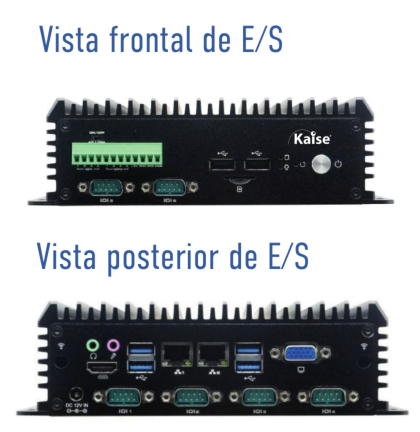
\includegraphics[width=.9\textwidth]{graficos/kaise}
    \end{minipage}
    \hfill
    \begin{minipage}[b]{0.48\textwidth}
        \begin{itemize}
            \item \textbf{Tipo:} PC industrial fanless compacta.
            \item \textbf{Procesador:} Intel Celeron J6412.
            \item \textbf{Memoria instalada:} 8~GB DDR4.
            \item \textbf{Red:} 2 interfaces Gigabit Ethernet.
            \item \textbf{Puertos E/S:} 6 puertos RS232 (2 RS485), \\2 USB 2.0, 4 USB 3.0, 8 GPIO. 
            \item \textbf{Alimentaci�n:} entrada DC de 12~V.
            \vspace{10px}
        \end{itemize}
    \end{minipage}
    \caption{Computadora principal embarcada para el control del sistema instrumental de la boya EAMMRA.}
    \label{fig:kaise}
\end{figure}

La elecci�n de una computadora industrial como unidad principal responde a la necesidad de integrar, en un �nico nodo de procesamiento, interfaces heterog�neas y tareas con distintos requerimientos temporales. A diferencia de una arquitectura basada exclusivamente en microcontroladores, esta soluci�n permite ejecutar un sistema operativo completo, utilizar bibliotecas de alto nivel para comunicaci�n con perif�ricos, mantener servicios de supervisi�n y registrar informaci�n en un sistema de archivos convencional. Esta capacidad resulta adecuada para una boya instrumental que debe combinar adquisici�n de sensores, control de perif�ricos, almacenamiento local, procesamiento preliminar de datos y preparaci�n de paquetes de telemetr�a bajo un r�gimen de operaci�n aut�nomo.

Desde el punto de vista funcional, la PC Kaise constituye el punto de convergencia entre el hardware de campo y la arquitectura de software del sistema. Las interfaces serie, USB, Ethernet y GPIO permiten vincular dispositivos con protocolos y velocidades de operaci�n diferentes, mientras que el entorno GNU/Linux facilita la separaci�n entre m�dulos de bajo nivel, servicios de control, rutinas de diagn�stico y procesos de almacenamiento. Esta organizaci�n favorece la mantenibilidad del sistema, simplifica la incorporaci�n de nuevos perif�ricos y permite ejecutar ensayos incrementales durante las etapas de integraci�n, validaci�n y operaci�n de la boya \citep{BoyaRepo}.

La disponibilidad de m�ltiples interfaces serie resulta especialmente relevante para la integraci�n simult�nea de perif�ricos. Asimismo, el dise�o sin ventilador reduce partes m�viles y mejora la aptitud del equipo para operaci�n embarcada.

\vspace{10px}
\subsection{Sensor ambiental AHT10.}

El AHT10 es un sensor digital de temperatura y humedad relativa utilizado para supervisar las condiciones ambientales internas o de entorno inmediato de la electr�nica de la boya. En EAMMRA se emplea como m�dulo comercial montado sobre una placa de circuito impreso auxiliar, lo que facilita su conexi�n el�ctrica, su fijaci�n mec�nica y su integraci�n al bus I2C de la computadora principal, como se observa en la Figura~\ref{fig:aht10}. La medici�n de temperatura y humedad no se incorpora como una variable oceanogr�fica principal, sino como una magnitud de diagn�stico para evaluar las condiciones de operaci�n del volumen donde se alojan los componentes electr�nicos.

\begin{figure}[htbp]
\centering
\begin{minipage}[b]{0.58\textwidth}
    \begin{itemize}
        \item \textbf{Variables medidas:} temperatura y humedad relativa.
        \item \textbf{Principio de medici�n:} elemento capacitivo MEMS para humedad y sensor de temperatura integrado.
        \item \textbf{Interfaz el�ctrica:} bus I2C.
        \item \textbf{Direcci�n I2C de referencia:} \texttt{0x38}.
        \item \textbf{Rango t�pico de humedad relativa:} 0 a 100~\%RH.
        \item \textbf{Rango t�pico de temperatura:} \(-40~^{\circ}\mathrm{C}\) a \(85~^{\circ}\mathrm{C}\).
        \item \textbf{Uso en la boya:} diagn�stico t�rmico y detecci�n de condiciones de humedad interna.
    \end{itemize}
\end{minipage}
\hfill
\begin{minipage}[b]{0.40\textwidth}
    \centering
    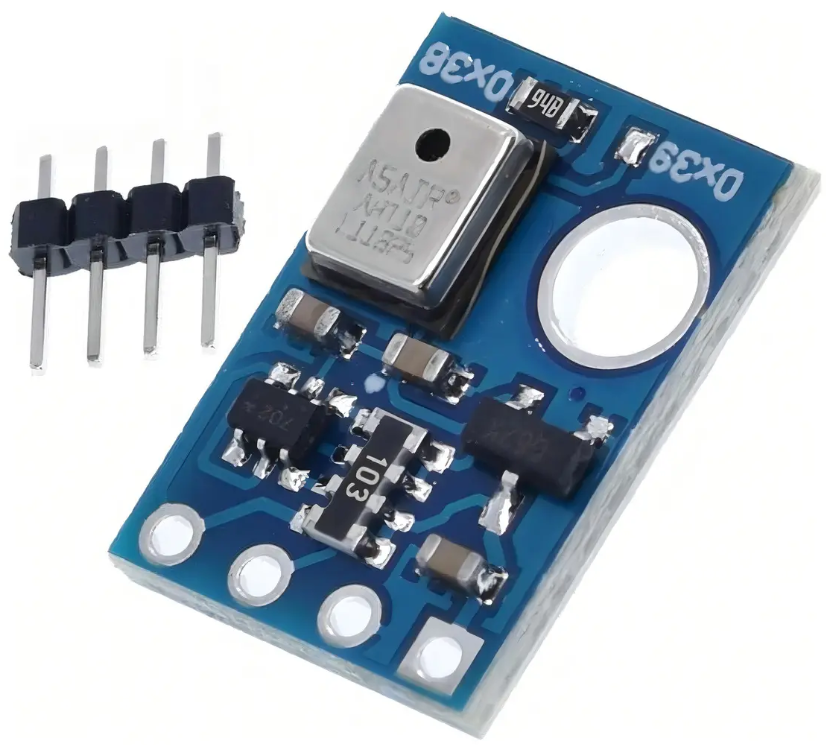
\includegraphics[width=0.5\linewidth]{graficos/aht10.png}
    \captionof{figure}{Sensor ambiental AHT10 utilizado para medici�n de temperatura y humedad relativa.}
    \label{fig:aht10}
\end{minipage}
\end{figure}

El sensor integra un elemento capacitivo MEMS sensible a la humedad relativa, un sensor de temperatura en chip y un circuito integrado de acondicionamiento y conversi�n \citep{AHT10Datasheet}. Esta arquitectura permite entregar una salida digital calibrada mediante una interfaz I2C est�ndar, sin requerir etapas anal�gicas externas de acondicionamiento. La disponibilidad de una medici�n digital resulta conveniente en un sistema embebido compacto, ya que reduce la cantidad de conexiones, evita la transmisi�n de se�ales anal�gicas de bajo nivel y simplifica la integraci�n con otros perif�ricos de supervisi�n.

Desde el punto de vista el�ctrico, el AHT10 requiere las l�neas de alimentaci�n, referencia de masa y las dos se�ales del bus I2C, SDA y SCL. Estas l�neas deben compartir una referencia com�n con la interfaz de adquisici�n y utilizar resistencias de \textit{pull-up} acordes al nivel l�gico del conjunto. En el montaje empleado, el sensor forma parte de un subconjunto USB--I2C junto con la unidad inercial, por lo que la longitud de las conexiones se mantiene reducida y el cableado queda contenido dentro del encapsulado local. Esta disposici�n disminuye la exposici�n de las se�ales digitales a interferencias y reduce la probabilidad de fallas por falsos contactos.

La ubicaci�n f�sica del sensor debe permitir el intercambio de aire con el volumen que se desea supervisar. Por este motivo, su protecci�n mec�nica debe equilibrar dos requisitos contrapuestos: por un lado, limitar la exposici�n directa a humedad condensada, salinidad, part�culas o contacto accidental; por otro, no aislar completamente el elemento sensible respecto del aire interno. En una plataforma mar�tima aut�noma, esta medici�n permite detectar condiciones que podr�an asociarse con ingreso de humedad, condensaci�n, degradaci�n del sellado o variaciones t�rmicas relevantes para la confiabilidad de la electr�nica.

Debe considerarse que los sensores de humedad relativa de este tipo pueden presentar deriva cuando operan durante per�odos prolongados en condiciones de humedad elevada o en presencia de vapores qu�micos. Por esta raz�n, en el sistema EAMMRA el AHT10 se utiliza principalmente como indicador de estado ambiental interno y no como instrumento meteorol�gico externo de referencia. Su valor reside en aportar una variable simple, de bajo consumo y bajo volumen f�sico, adecuada para el seguimiento de las condiciones de operaci�n del conjunto electr�nico embarcado.

\subsection{Unidad inercial MPU6050.}

El MPU6050 es una unidad inercial MEMS de seis grados de libertad que integra, en un mismo encapsulado, un aceler�metro triaxial y un gir�scopo triaxial. En EAMMRA se emplea como m�dulo comercial montado sobre una placa de circuito impreso auxiliar, que incorpora el sensor, los componentes pasivos necesarios para su operaci�n y los pines de conexi�n para alimentaci�n y comunicaci�n mediante bus I2C, como se observa en la Figura~\ref{fig:mpu6050}. 

Su funci�n dentro de la plataforma de hardware es registrar variables asociadas al movimiento local de la boya, con utilidad para diagn�stico mec�nico, identificaci�n de condiciones din�micas y contextualizaci�n de otros registros adquiridos por el sistema.

El aceler�metro mide aceleraciones lineales sobre tres ejes ortogonales, mientras que el gir�scopo mide velocidad angular alrededor de esos mismos ejes. Esta combinaci�n permite obtener una descripci�n local del movimiento de la estructura, sin requerir partes m�viles ni elementos mec�nicos externos. El dispositivo dispone de conversi�n digital interna y entrega las mediciones mediante una interfaz digital, lo que facilita su integraci�n con otros sensores de supervisi�n. Los rangos de escala completa del aceler�metro y del gir�scopo son seleccionables, lo que permite adecuar la sensibilidad del dispositivo a distintos niveles esperados de movimiento \citep{MPU6050Datasheet}.

\vspace{10px}
\begin{figure}[htbp]
\centering
\begin{minipage}[b]{0.29\textwidth}
    \centering
    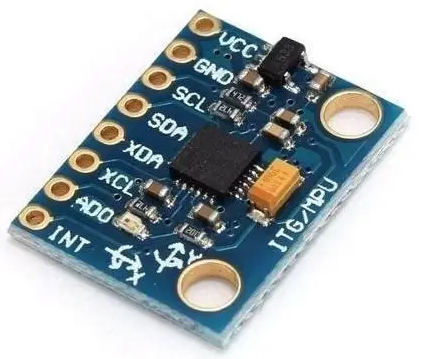
\includegraphics[width=0.90\linewidth]{graficos/mpu6050.png}
    \captionof{figure}{Unidad inercial MPU6050 para la medici�n de aceleraci�n y velocidad angular triaxial.}
    \label{fig:mpu6050}
\end{minipage}
\hfill
\begin{minipage}[b]{0.7\textwidth}
    \begin{itemize}
        \item \textbf{Variables medidas:} aceleraci�n y velocidad angular triaxial.
        \item \textbf{Tecnolog�a:} sensor inercial MEMS de seis grados de libertad.
        \item \textbf{Interfaz el�ctrica:} bus I2C.
        \item \textbf{Direcciones I2C posibles:} \texttt{0x68} y \texttt{0x69}.
        \item \textbf{Rangos aceler�metro:} \(\pm 2g\), \(\pm 4g\), \(\pm 8g\), \(\pm 16g\).
        \item \textbf{Rangos gir�scopo:} \(\pm 250\), \(\pm 500\), \(\pm 1000\), \(\pm 2000~^{\circ}/\mathrm{s}\).
        \item \textbf{Temperatura de operaci�n:} \(-40~^{\circ}\mathrm{C}\) a \(85~^{\circ}\mathrm{C}\).
        \item \textbf{Uso en la boya:} registro de movimiento y diagn�stico estructural.
    \end{itemize}
\end{minipage}
\end{figure}

Desde el punto de vista f�sico, la utilidad de la medici�n inercial depende de la fijaci�n mec�nica del m�dulo y de la orientaci�n de sus ejes respecto de la estructura de la boya. Para que las aceleraciones y velocidades angulares resulten interpretables, el sensor debe quedar firmemente vinculado al conjunto que se desea caracterizar, con m�nima holgura mec�nica y con una orientaci�n documentada durante la integraci�n. En particular, la presencia de cables sueltos, soportes flexibles o fijaciones deficientes puede introducir vibraciones locales que no representen adecuadamente el movimiento global de la plataforma.

El MPU6050 no constituye, por s� solo, un sistema de navegaci�n ni una referencia absoluta de actitud. Sus mediciones describen aceleraciones y velocidades angulares locales, afectadas por la orientaci�n del sensor, la respuesta din�mica del montaje, la temperatura y las vibraciones propias de la estructura. Por este motivo, en la boya se lo utiliza como sensor de diagn�stico y contexto din�mico, m�s que como instrumento de posicionamiento o navegaci�n. Esta funci�n es consistente con su integraci�n junto al sensor ambiental AHT10 en un subconjunto compacto de supervisi�n interna, conectado a la computadora principal mediante una interfaz USB--I2C.

\subsection{Integraci�n f�sica de sensores I2C mediante adaptador USB.}

Los sensores AHT10 y MPU6050 se integran a la computadora principal Kaise mediante un adaptador USB--I2C basado en CH431A. En la Figura~\ref{fig:ch431a} se muestra el adaptador utilizado como interfaz f�sica entre el puerto USB de la computadora embarcada y el bus I2C compartido por ambos sensores. 

A partir de las hojas de datos del AHT10 y del MPU6050 se verifican las condiciones el�ctricas de alimentaci�n, niveles l�gicos e interfaz digital requeridas para integrar ambos dispositivos en un mismo subconjunto de adquisici�n \citep{AHT10Datasheet,MPU6050Datasheet}.

La soluci�n adoptada reemplaza las conexiones desmontables de tipo Dupont por un montaje soldado, con el objetivo de reducir puntos de falla, mejorar la continuidad el�ctrica y aumentar la robustez frente a vibraciones, manipulaci�n durante la integraci�n y operaci�n embarcada. En este montaje, las l�neas SDA y SCL del bus I2C se distribuyen en com�n hacia ambos sensores, mientras que cada m�dulo conserva su propia direcci�n de dispositivo. La referencia de masa se comparte entre el adaptador y los sensores, y la alimentaci�n se toma del propio subconjunto USB--I2C, siempre dentro de los m�rgenes el�ctricos admitidos por los m�dulos empleados.

El conjunto de sensores se aloj� en un encapsulado \textit{ad-hoc} fabricado mediante impresi�n 3D. Este encapsulado cumple funciones de soporte, protecci�n y provee un anclaje mec�nico al disipador de la computadora Kaise. Posteriormente, se incorpor� resina epoxi para rigidizar el montaje y disminuir la exposici�n de contactos el�ctricos al ambiente interno de la boya. En el caso del AHT10, debe preservarse el intercambio de aire con el volumen que se desea supervisar, por lo que la protecci�n mec�nica no debe obturar completamente la zona sensible a humedad. En la  Figura~\ref{fig:conjunto-i2c-case-3d} se puede observar el conjunto y la ventana lateral donde se ubica el sensor AHT10.`

\begin{figure}[htbp]
\centering
\begin{minipage}[b]{0.47\textwidth}
    \centering
    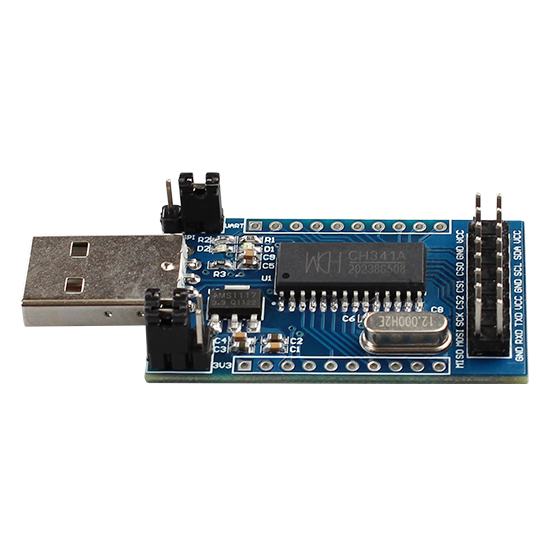
\includegraphics[width=0.70\linewidth]{graficos/ch431a.jpg}
    \captionof{figure}{Adaptador USB--I2C basado en CH431A utilizado para conectar los sensores AHT10 y MPU6050 a la omputadora principal.}
    \label{fig:ch431a}
\end{minipage}
\hfill
\begin{minipage}[b]{0.47\textwidth}
    \centering
    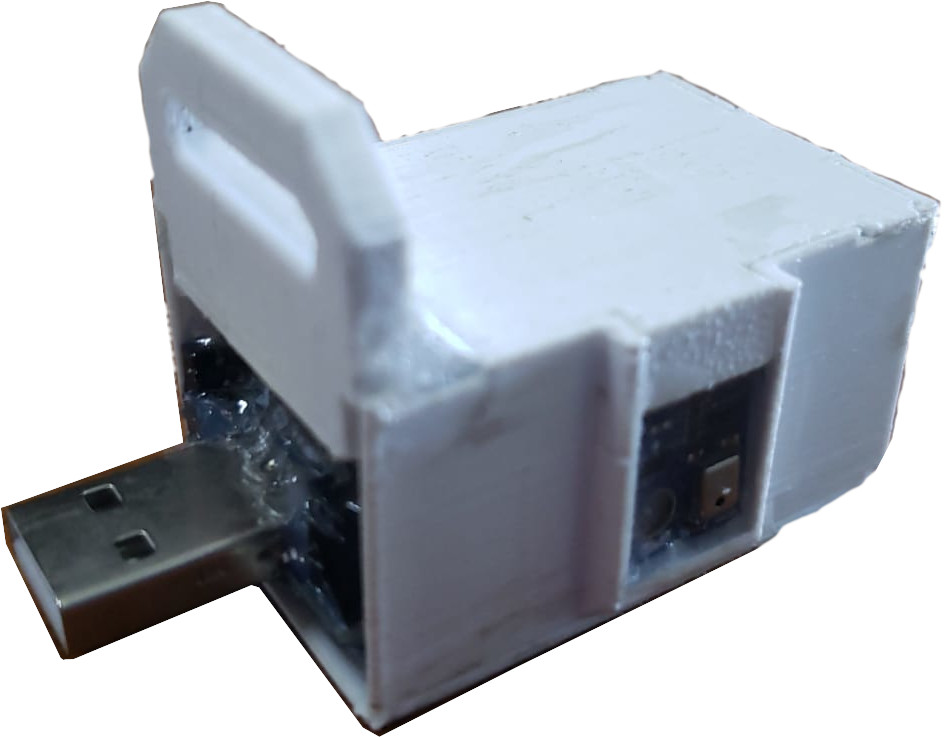
\includegraphics[width=0.65\linewidth]{graficos/conjunto_i2c_case_3d.jpeg}
    \captionof{figure}{Conjunto de sensores I2C integrado en un case \textit{ad-hoc} fabricado por impresi�n 3D y rigidizado mediante colada de resina epoxi.}
    \label{fig:conjunto-i2c-case-3d}
\end{minipage}
\end{figure}

Desde el punto de vista constructivo, esta integraci�n transforma m�dulos electr�nicos de desarrollo en un subconjunto m�s adecuado para operaci�n embarcada. La soldadura directa reduce la probabilidad de desconexi�n accidental, el encapsulado impreso mejora la fijaci�n mec�nica y la resina aporta estabilidad frente a vibraciones y manipulaci�n. Esta soluci�n tambi�n simplifica el reemplazo del conjunto completo durante tareas de mantenimiento, ya que concentra en un �nico dispositivo f�sico la medici�n ambiental provista por el AHT10 y la medici�n inercial provista por el MPU6050.

\subsection{Equipo AIS/GPS AMEC MANDO 301.}

El AMEC MANDO 301 se integra a la boya EAMMRA como equipo AIS AtoN, del ingl�s \emph{Automatic Identification System Aid to Navigation}, asociado al balizamiento electr�nico de la plataforma. Su funci�n principal es transmitir la identificaci�n y la posici�n de la boya mediante mensajes AIS, de modo que pueda ser detectada por embarcaciones cercanas y estaciones costeras compatibles. En la configuraci�n empleada, el equipo tambi�n aporta informaci�n GPS al sistema, lo que permite disponer de una referencia de posici�n y tiempo asociada a la operaci�n de la boya.

El MANDO 301 corresponde a un AIS AtoN tipo~1. Esta clase de equipo se caracteriza por operar como transmisor AIS, sin recepci�n de mensajes AIS de otras estaciones, y por utilizar acceso FATDMA, con ranuras temporales preasignadas para la emisi�n. En el caso de EAMMRA, el equipo no se utiliza para relevar tr�fico mar�timo circundante, sino para se�alizar electr�nicamente la presencia de la boya y proporcionar una referencia espacio-temporal para los registros adquiridos \citep{AMECMando301Brochure}.

En la Figura~\ref{fig:amec-mando-301} se muestra el equipo AMEC MANDO 301 junto con sus caracter�sticas principales de integraci�n. El dispositivo combina una interfaz de radiofrecuencia VHF para la transmisi�n AIS, una antena GPS externa para posicionamiento, alimentaci�n en corriente continua y puertos serie RS-232 para configuraci�n y comunicaci�n. Esta combinaci�n permite integrar el equipo tanto al subsistema de balizamiento como al sistema embebido de adquisici�n y supervisi�n.

\vspace{10px}
\begin{figure}[htbp]
\centering
\begin{minipage}[b]{0.34\textwidth}
\centering
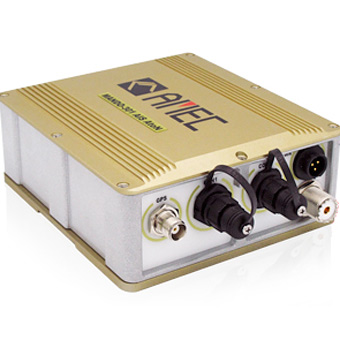
\includegraphics[width=0.90\linewidth]{graficos/amec_mando_301}
\captionof{figure}{Equipo AIS/GPS AMEC MANDO 301. Transmite identificaci�n y posici�n de la boya y aporta datos GPS al sistema embebido.}
\label{fig:amec-mando-301}
\end{minipage}
\hfill
\begin{minipage}[b]{0.62\textwidth}
\begin{itemize}
\item \textbf{Equipo:} AMEC MANDO 301, AIS AtoN tipo~1.
\item \textbf{Modo AIS:} transmisi�n FATDMA, sin recepci�n AIS.
\item \textbf{Funci�n AIS principal:} balizamiento electr�nico de ayudas a la navegaci�n.
\item \textbf{Posicionamiento:} receptor GPS con soporte SBAS y antena GPS externa.
\item \textbf{Interfaz de datos:} RS-232 a 115200~bit/s, 8N1.
\item \textbf{Interfaz RF:} antena VHF externa para transmisi�n AIS.
\item \textbf{Potencia de transmisi�n:} 2, 5 o 12,5~W, programable.
\item \textbf{Rol en EAMMRA:} identificaci�n, posicionamiento y balizamiento electr�nico.
\end{itemize}
\end{minipage}
\end{figure}
\vspace{10px}

Desde el punto de vista de la integraci�n f�sica, el equipo requiere una antena VHF externa adecuada para la banda AIS y una antena GPS externa ubicada con visibilidad suficiente hacia el cielo. La antena VHF condiciona el alcance efectivo de la se�al AIS, por lo que su montaje debe considerar altura, despeje, continuidad de masa, calidad del cable coaxial y protecci�n frente al ambiente mar�timo. La antena GPS, por su parte, permite al receptor interno obtener la posici�n de la boya y una referencia temporal derivada del sistema GNSS. Ambas antenas forman parte del sistema de se�alizaci�n y posicionamiento, y deben montarse de manera compatible con la geometr�a de la boya y con el resto de los subsistemas instalados en el m�stil o en la superestructura.

La alimentaci�n del MANDO 301 se realiza desde el sistema de energ�a de la boya, con tensi�n nominal de 12~VDC. Esta caracter�stica facilita su integraci�n con el banco de bater�as y el subsistema fotovoltaico. Adem�s de la conexi�n de potencia, el equipo dispone de conectores dedicados para configuraci�n, comunicaci�n, antena VHF y antena GPS. 

En t�rminos operativos, el aporte del MANDO 301 al sistema EAMMRA es doble. Por un lado, incrementa la seguridad de la plataforma al hacer visible la boya dentro del ecosistema AIS utilizado por embarcaciones y estaciones costeras. Por otro lado, proporciona datos de posici�n y tiempo que permiten asociar las mediciones ambientales, meteorol�gicas, energ�ticas y ac�sticas con una referencia espacial y temporal. 

\vspace{10px}



\subsection{Anem�metro ultras�nico WindSonic.}

El equipo WindSonic de Gill Instruments es un anem�metro ultras�nico de dos ejes utilizado para medir velocidad y direcci�n del viento. En la boya EAMMRA, este instrumento aporta informaci�n meteorol�gica de superficie que resulta relevante para la caracterizaci�n ambiental del sitio de medici�n y para el an�lisis posterior de las condiciones asociadas al ruido ambiente submarino. 

En la figura~\ref{fig:windsonic} se observa el anem�metro con sus dos pares de transductores perpendiculares que se utilizan para medir velocidad de viento a partir del tiempo de vuelo de pulsos ultras�nicos y luego se compone la direcci�n como una suma vectorial de cada eje.

\begin{figure}[htbp] 
	\centering 
	\begin{minipage}[c]{0.62\textwidth} 
		\begin{itemize} 
		\item \textbf{Variables medidas:} velocidad y direcci�n del viento. 
		\item \textbf{Principio de medici�n:} ultrasonido, sin partes m�viles. 
		\item \textbf{Rango de direcci�n:} 0 a 360 grados. 
		\item \textbf{Protocolos:} RS232 a 9600~bit/s, 8N1. 
		\item \textbf{Modo de adquisici�n:} \textit{polled}, a requerimiento.
		\item \textbf{Uso en EAMMRA:} caracterizaci�n meteorol�gica y correlaci�n con ruido ambiente submarino. 
		\end{itemize} 
	\end{minipage} 
	\hfill 
	\begin{minipage}[c]{0.35\textwidth} 
		\centering 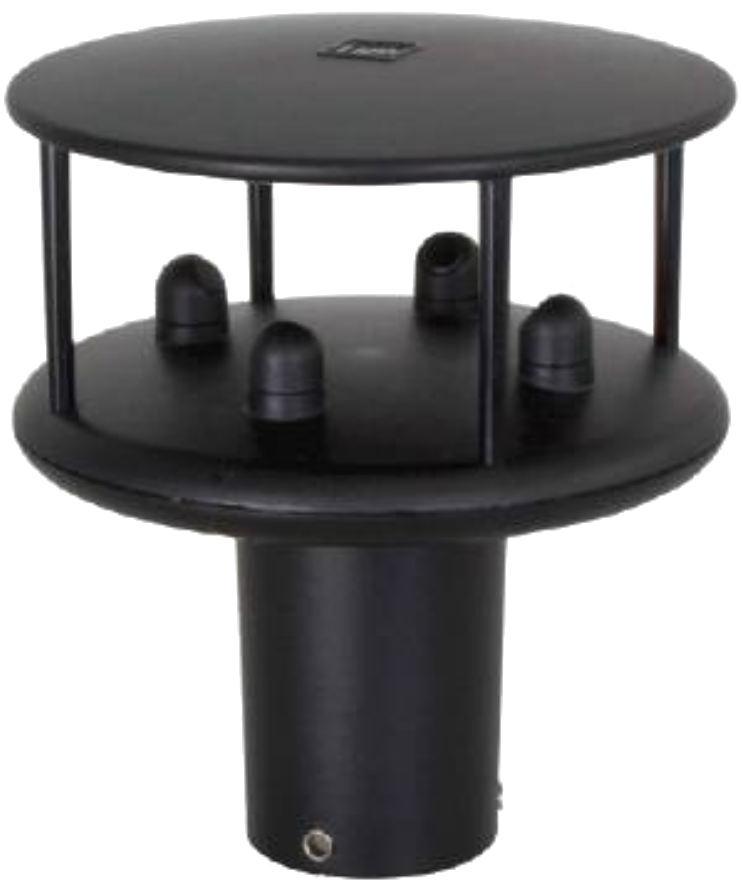
\includegraphics[width=0.6\linewidth]{graficos/anemometro.png} 
		\captionof{figure}{Anem�metro ultras�nico WindSonic utilizado para medir velocidad y direcci�n del viento.} 
		\label{fig:windsonic} 
	\end{minipage} 
\end{figure}

La integraci�n del WindSonic en EAMMRA y el desarrollo de las rutinas de configuraci�n, adquisici�n y registro fueron documentados previamente en el Informe T�cnico AS~1/24 \citep{RemottiBos2024_Anemometro}.

El sistema embebido se comunica con el instrumento mediante una conexi�n serie configurada a 9600~bit/s, 8N1. El modo de operaci�n empleado es de tipo solicitado, o \textit{polled}, por lo que el software de control debe requerir expl�citamente cada medici�n. El mensaje de respuesta incluye la direcci�n del viento, la velocidad, las unidades de medida, un c�digo de estado del instrumento y un campo de verificaci�n de integridad. Esta modalidad permite integrar la adquisici�n meteorol�gica dentro del ciclo general de operaci�n de la boya, sin depender de una transmisi�n continua no sincronizada con el resto de las tareas del sistema.

La conexi�n el�ctrica se realiza mediante el conector circular de 9 v�as provisto con el fabricante. Para la opci�n~1, el cableado combina dos conductores de alimentaci�n y tres conductores de comunicaci�n: transmisi�n, recepci�n y referencia de se�al. Como se muestra en la Figura~\ref{fig:windsonic-rs232}, la l�nea TXD del WindSonic se conecta con la entrada RXD del puerto serie o del conversor RS-232 a USB, mientras que la l�nea RXD del instrumento se conecta con la salida TXD de la interfaz de la computadora. La referencia com�n de se�al es necesaria para interpretar correctamente los niveles el�ctricos de la comunicaci�n serie. El blindaje del cable se conecta del lado de la computadora o del chasis, y no del lado del anem�metro, con el objetivo de reducir la susceptibilidad frente a interferencias el�ctricas sin introducir lazos de masa.

\begin{figure}[htbp]
 \centering
 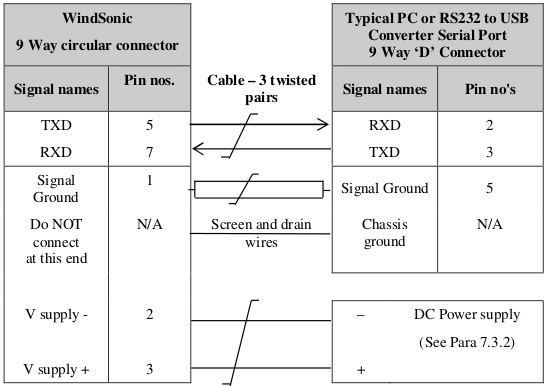
\includegraphics[width=0.7\linewidth]{graficos/windsonic_RS232.png}
 \captionof{figure}{Esquema de conexi�n RS-232 del anem�metro WindSonic, opci�n~1.}
 \label{fig:windsonic-rs232}
\end{figure}


\subsection{Controlador solar MPPT XTRA2210.}

El XTRA2210N es un controlador de carga solar de tipo MPPT, utilizado para administrar la transferencia de energ�a entre los paneles solares y el banco de bater�as de la boya. Su funci�n principal es regular el proceso de carga, proteger la bater�a y entregar al sistema embebido variables el�ctricas de supervisi�n. En EAMMRA, este perif�rico constituye el punto principal de observaci�n del subsistema energ�tico, ya que permite relevar par�metros asociados al arreglo fotovoltaico, la bater�a, la carga y el estado operativo del controlador.

La sigla MPPT corresponde a \emph{Maximum Power Point Tracking}, o seguimiento del punto de m�xima potencia. Un panel fotovoltaico no entrega su m�xima potencia para cualquier combinaci�n de tensi�n y corriente, sino en un punto particular de su curva caracter�stica \(I\)-\(V\). Ese punto depende de la irradiancia, la temperatura del panel, el estado de carga de la bater�a y las condiciones instant�neas de operaci�n. El controlador MPPT modifica din�micamente el punto de trabajo el�ctrico del panel para operar cerca de la potencia m�xima disponible y luego adapta esa energ�a a las condiciones requeridas por la bater�a mediante una etapa de conversi�n DC/DC.

El controlador solar MPPT XTRA2210N se muestra en la Figura~\ref{fig:xtra2210}. Sus caracter�sticas principales se resumen junto a la imagen del equipo.

\begin{figure}[htbp]
    \centering
    \begin{minipage}[b]{0.34\textwidth}
        \centering
        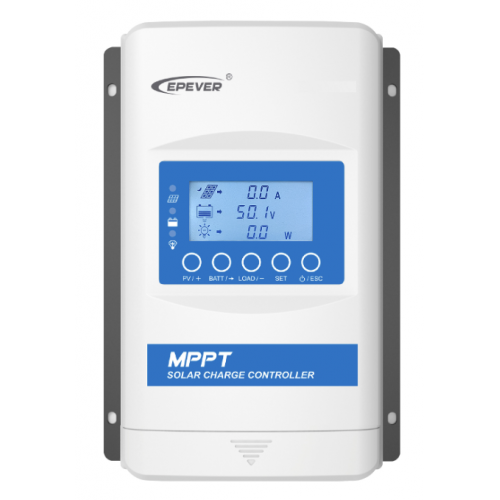
\includegraphics[width=0.90\linewidth]{graficos/xtra2210.png}
        \captionof{figure}{Controlador solar MPPT XTRA2210N utilizado para la gesti�n y supervisi�n energ�tica de la boya EAMMRA.}
        \label{fig:xtra2210}
    \end{minipage}
    \hfill
    \begin{minipage}[b]{0.62\textwidth}
        \begin{itemize}
            \item \textbf{Modelo:} XTRA2210N, familia XTRA-N.
            \item \textbf{Tipo:} controlador de carga solar MPPT.
            \item \textbf{Corriente nominal de carga:} 20~A.
            \item \textbf{Tensi�n nominal del sistema:} 12/24~V.
            \item \textbf{Interfaz de comunicaci�n:} RS485.
            \item \textbf{Protocolo:} Modbus.
            \item \textbf{Funci�n principal:} gesti�n de carga entre paneles solares y banco de bater�as.
            \item \textbf{Uso en EAMMRA:} supervisi�n energ�tica y diagn�stico del sistema fotovoltaico.
        \end{itemize}
    \end{minipage}
\end{figure}

Este controlador se diferencia de los controladores PWM. En un regulador PWM, el panel queda acoplado en forma m�s directa al banco de bater�as durante la etapa de carga. Por esta raz�n, la tensi�n de operaci�n del arreglo fotovoltaico tiende a quedar limitada por la tensi�n instant�nea de la bater�a. Como consecuencia, el panel puede operar lejos de su punto de m�xima potencia, especialmente cuando existe una diferencia significativa entre la tensi�n �ptima del panel y la tensi�n de la bater�a. En cambio, un controlador MPPT permite que el panel opere a una tensi�n m�s conveniente desde el punto de vista energ�tico y convierte la diferencia de tensi�n en mayor corriente de carga.

Para una boya instrumental aut�noma, esta diferencia es relevante. La energ�a disponible condiciona la frecuencia de adquisici�n, la disponibilidad de telemetr�a, el tiempo de operaci�n continua y la capacidad de recuperaci�n despu�s de per�odos de baja irradiancia. El uso de un controlador MPPT permite mejorar el aprovechamiento del arreglo fotovoltaico, ampliar el margen energ�tico del sistema y disponer de variables de diagn�stico para evaluar el estado de la alimentaci�n durante la operaci�n.


La diferencia funcional entre controladores PWM y MPPT se sintetiza en la Tabla~\ref{tab:pwm-mppt}. En el contexto de EAMMRA, la alternativa MPPT resulta m�s adecuada porque mejora el aprovechamiento energ�tico disponible y permite obtener variables de supervisi�n �tiles para la operaci�n aut�noma.

\begin{table}[htbp]
\centering
\small
\setlength{\tabcolsep}{4pt}
\renewcommand{\arraystretch}{1.18}

\caption{Comparaci�n conceptual entre controladores solares PWM y MPPT.}
\label{tab:pwm-mppt}

\begin{tabular}{p{0.24\textwidth}p{0.35\textwidth}p{0.35\textwidth}}
    \hline
    \textbf{Caracter�stica} &
    \textbf{PWM} &
    \textbf{MPPT} \\
    \hline

    Punto de operaci�n del panel &
    Vinculado en forma directa a la tensi�n instant�nea de la bater�a. &
    Ajustado para operar cerca del punto de m�xima potencia del panel. \\

    Conversi�n de energ�a &
    No realiza adaptaci�n DC/DC optimizada entre panel y bater�a. &
    Utiliza conversi�n DC/DC para adaptar tensi�n y corriente de carga. \\

    Aprovechamiento energ�tico &
    Menor cuando la tensi�n �ptima del panel difiere de la tensi�n de bater�a. &
    Mayor aprovechamiento del arreglo fotovoltaico en condiciones variables. \\

    Complejidad electr�nica &
    Baja, con arquitectura m�s simple. &
    Mayor, debido al seguimiento del punto de m�xima potencia y a la etapa de conversi�n. \\

    Costo relativo &
    Generalmente menor. &
    Generalmente mayor. \\

    Adecuaci�n a EAMMRA &
    Limitada para una plataforma aut�noma con presupuesto energ�tico restringido. &
    M�s adecuada para maximizar autonom�a y supervisar variables el�ctricas del sistema. \\

    \hline
\end{tabular}

\end{table}



Adem�s de su funci�n de carga, el XTRA2210N aporta informaci�n �til para el software de control mediante comunicaci�n serie RS485 con protocolo Modbus. Entre las variables de inter�s se incluyen tensi�n y corriente del panel, tensi�n y corriente de bater�a, potencia de carga, temperatura de bater�a, temperatura interna del dispositivo, estado de carga estimado y estados de protecci�n o falla. Estas mediciones permiten registrar la evoluci�n energ�tica de la boya, detectar condiciones an�malas y correlacionar el estado de energ�a con la ejecuci�n de tareas de adquisici�n, procesamiento y transmisi�n satelital.

En t�rminos funcionales, el controlador cumple cuatro roles dentro de EAMMRA: maximiza la energ�a extra�da de los paneles solares, regula la carga del banco de bater�as, protege el sistema frente a condiciones el�ctricas no deseadas y provee telemetr�a energ�tica al sistema embebido. Por este motivo, no se lo considera s�lo un componente de potencia, sino tambi�n un perif�rico de supervisi�n esencial para la operaci�n aut�noma de la boya.

\subsection{Subsistema ac�stico.}

El subsistema ac�stico constituye la cadena principal de adquisici�n cient�fica de la boya EAMMRA. Su funci�n es convertir el campo de presi�n ac�stica submarina en se�ales el�ctricas, acondicionarlas mediante una etapa anal�gica de bajo ruido y digitalizarlas mediante una placa de adquisici�n de audio conectada a la computadora principal. Desde el punto de vista de hardware, la cadena est� compuesta por dos hidr�fonos anal�gicos calibrados Br{"u}el \& Kj{\ae}r 8105, dos preamplificadores para hidr�fonos desarrollados por la Divisi�n Ac�stica Submarina y una placa de audio USB Behringer UMC202HD.

La arquitectura de adquisici�n responde a una separaci�n funcional entre transducci�n, acondicionamiento y digitalizaci�n. Los hidr�fonos convierten las variaciones de presi�n ac�stica en tensi�n el�ctrica; los preamplificadores adaptan la impedancia, elevan el nivel de se�al y limitan componentes de baja frecuencia capaces de saturar la etapa posterior; finalmente, la placa de audio digitaliza dos canales en forma simult�nea y entrega los datos a la computadora principal mediante USB. Esta organizaci�n permite utilizar sensores ac�sticos calibrados y preservar una cadena instrumental verificable, con etapas diferenciadas para medici�n, acondicionamiento y conversi�n anal�gico-digital.

\vspace{10pt}

\noindent \textbf{Hidr�fonos Br{"u}el \& Kj{\ae}r 8105.}

Los sensores utilizados para captar las se�ales ac�sticas son dos hidr�fonos anal�gicos calibrados Br{"u}el \& Kj{\ae}r, modelo 8105. Se trata de transductores piezoel�ctricos cer�micos, sin preamplificaci�n interna, adecuados para mediciones de banda ancha en ambiente submarino. Su selecci�n se justifica por su ancho de banda, sensibilidad, comportamiento omnidireccional y aptitud mec�nica para operaci�n sumergida \citep{byk}. En la Figura~\ref{fig:8105} se presentan las dimensiones mec�nicas principales del hidr�fono junto con las caracter�sticas t�cnicas m�s relevantes para su integraci�n en EAMMRA.

\vspace{20px}
\begin{figure}[htbp]
\centering
\begin{minipage}[b]{0.42\textwidth}
\centering
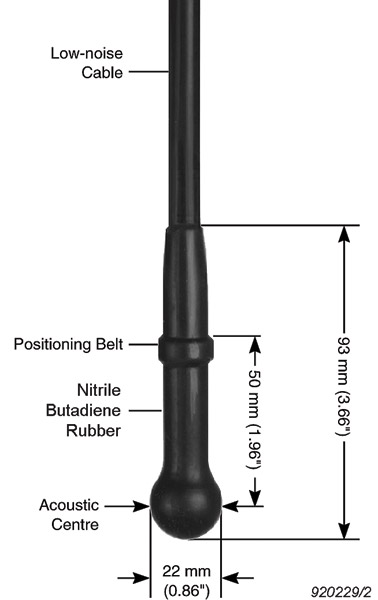
\includegraphics[height=.30\textheight]{graficos/8105.jpg}
\captionof{figure}{Dimensiones mec�nicas del hidr�fono Br{"u}el \& Kj{\ae}r modelo 8105.}
\label{fig:8105}
\end{minipage}
\hfill
\begin{minipage}[b]{0.54\textwidth}
\begin{itemize}
\item \textbf{Modelo:} Br{"u}el \& Kj{\ae}r 8105.
\item \textbf{Tipo:} hidr�fono anal�gico piezoel�ctrico calibrado.
\item \textbf{Rango de frecuencia:} 0.1~Hz a 160~kHz.
\item \textbf{Sensibilidad nominal:} (-205)~dB re 1~V/($\mu$)Pa.
\item \textbf{Directividad:} omnidireccional en su rango operativo.
\item \textbf{Presi�n hidrost�tica admisible:} 9.8~MPa, aproximadamente 1000~m de profundidad.
\item \textbf{Protecci�n externa:} recubrimiento polim�rico apto para operaci�n en medio marino.
\item \textbf{Conexi�n:} cable sumergible integrado, con terminaci�n BNC no sumergible.
\end{itemize}
\end{minipage}
\end{figure}

Las curvas de respuesta en frecuencia y las caracter�sticas particulares de cada hidr�fono utilizado en la boya est�n dadas por las respectivas hojas de calibraci�n provistas por el fabricante. En dichas calibraciones se considera el efecto del cable integrado al elemento sensor, cuyo aporte capacitivo modifica la impedancia vista desde el terminal de conexi�n. Los hidr�fonos adquiridos para el desarrollo poseen longitudes de cable de 50~m y 20~m, respectivamente.

El cable integrado al hidr�fono es sumergible, de tipo \textit{waterblocked}, grado militar DSS-2, especificado en el est�ndar MIL-DTL-915/8 \citep{mil-std:dtl-915}. Se trata de un cable flexible, aislado y blindado, de dos conductores, apto para electr�nica, comunicaciones e instrumentaci�n en equipamiento embarcado. Los cables de ambos hidr�fonos finalizan en conectores BNC no sumergibles, por lo que la integraci�n mec�nica y el�ctrica debe garantizar protecci�n adecuada dentro de la boya y evitar la exposici�n directa del conector al ambiente marino.

\vspace{10pt}

\noindent \textbf{Preamplificadores DAS-1/DAS-2.}

Debido a que los hidr�fonos B\&K 8105 no poseen preamplificaci�n interna, las se�ales el�ctricas generadas pueden presentar amplitudes muy bajas frente al ruido propio de la etapa de adquisici�n. Adem�s, vistos desde sus terminales de salida, los hidr�fonos se comportan como fuentes de alta impedancia con una componente capacitiva significativa. Esta condici�n exige una etapa de acondicionamiento anal�gico con muy alta impedancia de entrada, bajo ruido propio y ancho de banda compatible con el rango de medici�n previsto.

Como parte de los desarrollos previos de EAMMRA, se dise�� y fabric� un preamplificador espec�fico para hidr�fonos B\&K 8105, orientado a trabajar con cargas capacitivas y con un ancho de banda aproximado de 100~kHz \citep{AS0518_Preamp}. El dise�o se bas� en amplificadores operacionales de bajo ruido LT1792, en configuraci�n no inversora, con alimentaci�n dual generada a partir de una fuente principal de tipo \textit{single supply}. En la configuraci�n actual de la boya se utilizan dos unidades de preamplificaci�n, denominadas DAS-1 y DAS-2. En la Figura~\ref{fig:preamp-das} se muestra una de las unidades utilizadas junto con sus caracter�sticas principales de integraci�n.

\vspace{20px}
\begin{figure}[htbp]
\centering
\begin{minipage}[b]{0.36\textwidth}
\centering
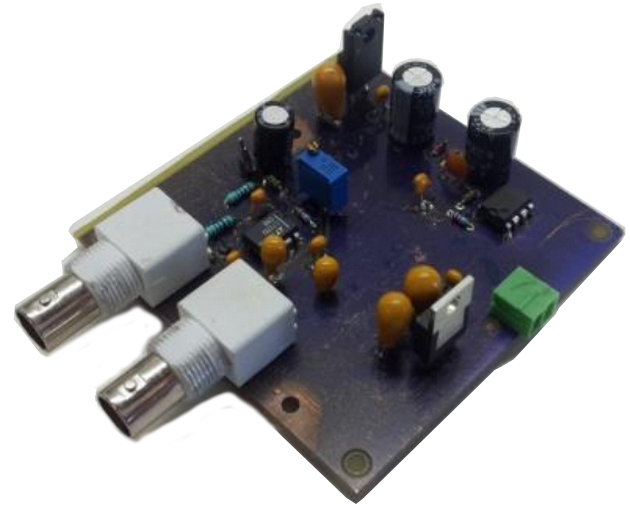
\includegraphics[width=\linewidth]{graficos/preamp_definitivo.jpg}
\captionof{figure}{Preamplificador para hidr�fonos DAS utilizado en la cadena ac�stica de EAMMRA.}
\label{fig:preamp-das}
\end{minipage}
\hfill
\begin{minipage}[b]{0.60\textwidth}
\begin{itemize}
\item \textbf{Identificaci�n:} preamplificadores DAS-1 y DAS-2.
\item \textbf{Aplicaci�n:} acondicionamiento de B\&K 8105.
\item \textbf{Topolog�a:} amplificador no inversor de bajo ruido.
\item \textbf{Amplificador operacional:} LT1792.
\item \textbf{Ganancia nominal:} aproximadamente 40~dB.
\item \textbf{Respuesta en frecuencia:} hasta 100~kHz.
\item \textbf{Entrada:} adaptada a cargas capacitivas del orden de nF.
\item \textbf{Protecci�n funcional:} corte en bajas frecuencias para reducir saturaci�n por componentes de gran amplitud.
\item \textbf{Alimentaci�n:} entrada principal entre 9~V y 15~V, con generaci�n local de tensi�n negativa.
\end{itemize}
\end{minipage}
\end{figure}

\vspace{20px}

La etapa de preamplificaci�n cumple tres funciones principales. En primer lugar, eleva la amplitud de las se�ales generadas por los hidr�fonos para que superen el ruido propio de la placa de adquisici�n. En segundo lugar, presenta una impedancia de entrada adecuada para evitar una carga excesiva sobre el hidr�fono y preservar la respuesta de la cadena. En tercer lugar, incorpora un corte en bajas frecuencias que aten�a componentes de gran amplitud capaces de saturar la etapa de digitalizaci�n. Esta �ltima condici�n resulta importante en registros de ruido ambiente, donde pueden coexistir se�ales de baja frecuencia con niveles elevados y componentes de inter�s en bandas superiores.

\vspace{10pt}

\noindent \textbf{Placa de audio Behringer UMC202HD.}

La digitalizaci�n de la se�al acondicionada se realiza mediante una placa de audio USB Behringer UMC202HD. Esta placa proporciona dos canales de adquisici�n simult�nea, frecuencia de muestreo de hasta 192~kHz por canal y resoluci�n nominal de 24~bits. En la boya, la placa act�a como interfaz entre la cadena anal�gica hidr�fono-preamplificador y la computadora principal. En la Figura~\ref{fig:behringer-umc202hd} se presenta la placa utilizada y se resumen sus caracter�sticas principales.

\vspace{20px}
\begin{figure}[htbp]
\centering
\begin{minipage}[c]{0.36\textwidth}
\centering
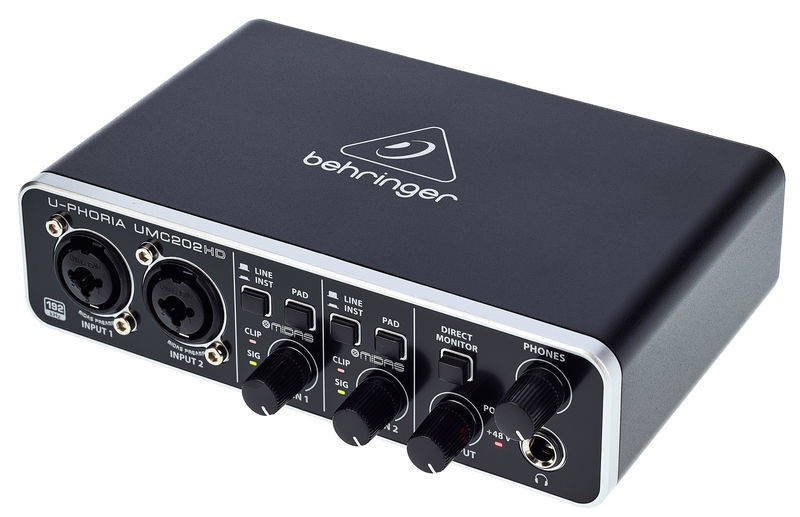
\includegraphics[width=\linewidth]{graficos/behringer_umc202hd.png}
\captionof{figure}{Placa de audio Behringer UMC202HD utilizada para la digitalizaci�n de se�ales ac�sticas.}
\label{fig:behringer-umc202hd}
\end{minipage}
\hfill
\begin{minipage}[c]{0.60\textwidth}
\begin{itemize}
\item \textbf{Modelo:} Behringer UMC202HD.
\item \textbf{Tipo:} placa de audio USB.
\item \textbf{Canales:} 2 entradas de adquisici�n simult�nea.
\item \textbf{Frecuencia de muestreo m�xima:} 192~kHz por canal.
\item \textbf{Resoluci�n nominal:} 24~bits.
\item \textbf{Uso en EAMMRA:} digitalizaci�n de se�ales ac�sticas provenientes de los preamplificadores DAS-1/DAS-2.
\end{itemize}
\end{minipage}
\end{figure}

La caracterizaci�n del conjunto placa-preamplificador se documenta en la Nota T�cnica AS~02/26 \citep{Cinquini2026_AS0226}. En dicho trabajo se relevaron la respuesta en frecuencia de la placa de audio, la respuesta de los preamplificadores DAS-1 y DAS-2, la figura de ruido propio y el crosstalk entre canales. Los resultados obtenidos permitieron verificar que la cadena de adquisici�n ac�stica es compatible con el uso previsto en EAMMRA y que el hardware de adquisici�n no constituye un limitante para la medici�n de niveles de ruido ambiente submarino dentro del rango operativo considerado.

En conjunto, el subsistema ac�stico queda definido como una cadena instrumental calibrable y modular. Los hidr�fonos establecen la sensibilidad primaria frente al campo ac�stico submarino, los preamplificadores adecuan la se�al a los niveles requeridos por la etapa de digitalizaci�n y la placa de audio convierte ambos canales en datos digitales disponibles para la computadora principal. Esta separaci�n por etapas facilita la verificaci�n individual de componentes, la trazabilidad de la cadena de medici�n y el mantenimiento del sistema durante la operaci�n de la boya.

\subsection{M�dem satelital Iridium SBD.}

El subsistema Iridium proporciona el enlace de telemetr�a satelital de la boya EAMMRA mediante el servicio \textit{Short Burst Data} (SBD). Este servicio est� orientado a la transmisi�n bidireccional de mensajes cortos entre equipos remotos y sistemas centrales, por lo que resulta adecuado para plataformas aut�nomas con bajo volumen de datos transmitidos y operaci�n fuera de cobertura celular o infraestructura costera \citep{IridiumSBDService}. En la boya, el enlace satelital se utiliza para transmitir informaci�n compacta de estado, diagn�stico y resultados seleccionados, sin reemplazar al almacenamiento local de datos completos.

La familia de transceptores Iridium 9603/9603N constituye una referencia t�cnica representativa para este tipo de integraci�n. Estos m�dulos est�n dise�ados como transceptores SBD de placa �nica, destinados a incorporarse dentro de un sistema anfitri�n que provee alimentaci�n, l�gica de control, antena y acondicionamiento de interfaces. El transceptor no implementa voz, datos conmutados por circuito ni SMS, sino exclusivamente comunicaci�n SBD. Esta caracter�stica es consistente con el uso previsto en EAMMRA, donde la telemetr�a se limita a mensajes breves y seleccionados \citep{Iridium9603NDevGuide}. En la Figura~\ref{fig:iridium} se muestra el m�dem satelital Iridium utilizado como perif�rico de telemetr�a remota.

\begin{figure}[htbp]
\centering
\begin{minipage}[b]{0.36\textwidth}
\centering
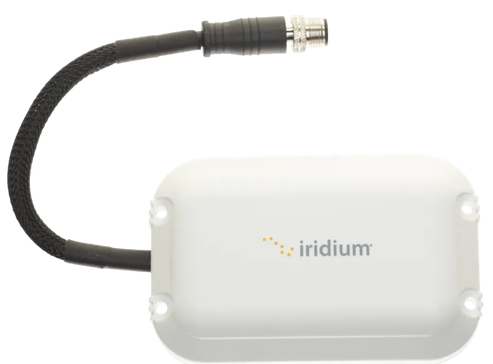
\includegraphics[width=0.90\linewidth]{graficos/iridium.png}
\captionof{figure}{M�dem satelital Iridium utilizado para telemetr�a remota mediante el servicio SBD.}
\label{fig:iridium}
\end{minipage}
\hfill
\begin{minipage}[b]{0.60\textwidth}
\begin{itemize}
\item \textbf{Servicio:} Iridium Short Burst Data.
\item \textbf{Tipo de enlace:} comunicaci�n satelital en banda L.
\item \textbf{Mensajes:} \textit{Mobile Originated} y \textit{Mobile Terminated}.
\item \textbf{Interfaz de control:} puerto serie con comandos AT.
\item \textbf{Interfaz RF:} antena externa para banda Iridium.
\item \textbf{Impedancia nominal de antena:} 50~($\Omega$).
\item \textbf{Funci�n en EAMMRA:} transmisi�n remota de estado, diagn�stico y resultados compactos.
\end{itemize}
\end{minipage}
\end{figure}



Desde el punto de vista el�ctrico, la integraci�n del m�dem requiere considerar dos aspectos principales: la interfaz serie de control y la alimentaci�n durante los ciclos de transmisi�n. El transceptor 9603/9603N utiliza una interfaz serie de tipo DCE hacia la aplicaci�n anfitriona y transfiere comandos, respuestas y datos SBD mediante comandos AT. Si el sistema anfitri�n emplea niveles RS-232 convencionales, debe incorporarse la adaptaci�n de niveles correspondiente. 

La antena satelital constituye un elemento cr�tico del enlace. Debe estar ubicada con una vista despejada del cielo y con m�nima obstrucci�n por la estructura de la boya, el m�stil u otros perif�ricos instalados. El tramo de RF entre el m�dem y la antena debe mantener la impedancia adecuada, minimizar p�rdidas y utilizar conectores y cable coaxial compatibles con operaci�n en ambiente mar�timo. En t�rminos de dise�o f�sico, la instalaci�n debe proteger conectores, evitar esfuerzos mec�nicos sobre el cableado y asegurar una puesta a masa coherente con el resto de la electr�nica embarcada.

El uso de SBD impone una restricci�n deliberada sobre el volumen de informaci�n transmitida. Por esta raz�n, el enlace satelital se reserva para datos resumidos y de alto valor operativo, tales como estado general del sistema, continuidad de operaci�n, condiciones energ�ticas, disponibilidad de almacenamiento, posici�n, diagn�stico de perif�ricos y resultados compactos derivados de mediciones ac�sticas. Los archivos completos, en particular los registros WAV y los datos de mayor volumen, permanecen almacenados localmente en la boya.

En conjunto, el m�dem Iridium SBD se incorpora como perif�rico de comunicaci�n remota de baja tasa de datos y alta cobertura geogr�fica. Su valor dentro de EAMMRA no reside en transportar grandes vol�menes de informaci�n, sino en permitir seguimiento remoto, verificaci�n de continuidad operativa y recuperaci�n parcial de informaci�n cr�tica durante campa�as prolongadas. Esta funci�n complementa el almacenamiento local y proporciona una v�a de supervisi�n externa cuando la boya opera fuera del alcance de redes terrestres.

\vspace{20px}
\subsection{Almacenamiento local.}

La boya EAMMRA incorpora almacenamiento local mediante una unidad de estado s�lido de 1~TB. Este dispositivo constituye el soporte primario para conservar los datos cient�ficos y operativos adquiridos durante una campa�a. La telemetr�a satelital Iridium SBD permite transmitir informaci�n compacta de estado, diagn�stico y resultados seleccionados, pero no est� destinada al env�o de archivos de gran volumen. Por este motivo, los registros completos, en particular los archivos ac�sticos, permanecen almacenados en la boya hasta su recuperaci�n durante tareas de mantenimiento o al finalizar la operaci�n.

La elecci�n de una unidad SSD resulta adecuada para una plataforma mar�tima aut�noma. A diferencia de un disco r�gido mec�nico, un SSD no posee partes m�viles, presenta mayor tolerancia frente a vibraciones y movimientos, y reduce el riesgo de fallas asociadas a golpes durante maniobras de despliegue, recuperaci�n o transporte. Adem�s, su bajo volumen f�sico y su consumo moderado facilitan la integraci�n dentro del gabinete electr�nico de la boya, junto con la computadora principal y los perif�ricos de adquisici�n.

El almacenamiento local concentra informaci�n de distinta naturaleza. Los archivos ac�sticos WAV constituyen el conjunto de datos de mayor volumen y representan el registro primario del subsistema ac�stico. Junto con ellos se almacenan mediciones meteorol�gicas del anem�metro WindSonic, variables ambientales internas provistas por el AHT10, variables inerciales medidas por el MPU6050, par�metros energ�ticos del controlador solar MPPT, datos de posici�n y tiempo, registros de eventos, mensajes de diagn�stico y mensajes de telemetr�a generados o pendientes de transmisi�n.

El volumen de almacenamiento requerido est� dominado por la adquisici�n ac�stica. Para una se�al digital de $N_c$ canales, frecuencia de muestreo $f_s$ y $N_b$ bytes por muestra, el flujo ideal de datos puede estimarse como:

\begin{equation}
R = N_c \cdot f_s \cdot N_b
\label{eq:flujo-datos-acusticos}
\end{equation}

En una configuraci�n de dos canales, frecuencia de muestreo de 192~kHz y resoluci�n de 24~bits, equivalente a 3~bytes por muestra, el flujo resultante es aproximadamente 1.15~MB/s. Esto corresponde a unos 4.15~GB/h, o cerca de 100~GB por d�a de adquisici�n continua. Por lo tanto, una unidad de 1~TB permite almacenar del orden de varios d�as de audio continuo a m�xima tasa, y un per�odo mayor cuando la adquisici�n se organiza en ventanas temporales o con frecuencias de muestreo menores. Si el formato de almacenamiento utiliza palabras de 32~bits por muestra, el volumen diario aumenta en forma proporcional.



Adem�s de la capacidad nominal, el almacenamiento local debe considerarse como parte de la confiabilidad operativa del sistema. La boya puede experimentar reinicios, interrupciones de energ�a o apagados controlados durante per�odos de baja disponibilidad energ�tica. Por este motivo, el uso del SSD debe complementarse con criterios de escritura robusta, cierre ordenado de archivos y separaci�n entre datos cient�ficos, registros de estado y mensajes de telemetr�a. Esta organizaci�n facilita la recuperaci�n posterior de la informaci�n y permite reconstruir la secuencia de operaci�n de la boya ante eventos an�malos.

En conjunto, el SSD de 1~TB act�a como memoria persistente principal del sistema embebido. Su funci�n es preservar la totalidad de los datos de campa�a, mientras que la telemetr�a satelital proporciona una v�a de supervisi�n remota limitada a informaci�n compacta. Esta separaci�n entre almacenamiento local de alto volumen y transmisi�n remota de baja tasa permite compatibilizar la adquisici�n ac�stica de alta demanda con la operaci�n aut�noma y energ�ticamente restringida de la boya.


\clearpage
\section{Dise�o e Implementaci�n}
\label{sec:diseno_e_implementacion}
\subsection{Arquitectura del sistema}
\subsection{Proceso principal y enrutamiento de eventos}
\subsection{Planificador y gesti�n de tareas}
\subsection{M�dulos de sensores}
\subsubsection{Sensores ambientales (AHT10, MPU6050)}
\subsubsection{Sensores meteorol�gicos y de posici�n}
\subsubsection{Procesamiento de audio}
\subsubsection{Gesti�n de energ�a}
\subsection{Telemetr�a satelital (Iridium SBD)}
\subsection{Protocolos y formatos de datos}
\subsection{Almacenamiento y pol�ticas de persistencia}

\section{Pruebas y Ensayos}
\subsection{Pruebas unitarias y de integraci�n}
\subsection{Tests de bajo nivel y simulaciones (mocks)}
\subsection{Ensayos operacionales en laboratorio}
\subsection{Pruebas de campo y telemetr�a}
\subsection{Resultados obtenidos}

\section{Conclusiones y Trabajo Futuro}
\subsection{Conclusiones}
\subsection{Logros alcanzados}
\subsection{Dificultades encontradas y lecciones aprendidas}
\subsection{Trabajo futuro}
\subsubsection{Mejoras propuestas}
\subsubsection{Nuevas funcionalidades}
\subsubsection{Escalabilidad y mantenimiento del sistema}


% =====================================================================================================
% =====================================================================================================
% PÁGINA DE REFERENCIAS
% =====================================================================================================
% =====================================================================================================

\clearpage
\vspace{4pc}
\addcontentsline{toc}{section}{REFERENCIAS}
\bibliographystyle{apa-good}	% (uses file "plain.bst")
\bibliography{7_Referencias}	% Acá está la base de datos de referencias. Espera el archivo "7_Referencias.bib"

\clearpage

% =====================================================================================================
% =====================================================================================================
% APÉNDICE
% =====================================================================================================
% =====================================================================================================


% Reseteo y cambio de numeración para los apéndices
\setcounter{section}{0}
\renewcommand\appendix{\Roman{section}}
%\def\thesection{\Roman{section}}

% =================================================================================================
% =================================================================================================
%\appendix
% =================================================================================================
% =================================================================================================
\appendix
\appendixpage
\addappheadtotoc
\section{Pseudocódigo de software embebido}
\label{ap:pseudocodigo_software}

En este apéndice se reúnen los listados de pseudocódigo asociados a la arquitectura de software. Su objetivo es documentar el flujo lógico de operación sin interrumpir la descripción principal del diseño.

\subsection{Modelo de ejecución}

\begin{lstlisting}[
    style=pseudocodigo,language=Python, caption={Pseudocódigo del modelo de ejecución del sistema embebido.}, label={lst:modelo_ejecucion}]
    
def main():
    config = cargar_configuracion()

    colas_entrada = crear_colas_entrada(config.modulos)
    cola_estado = crear_cola_estado()

    modulos = instanciar_fsm(config.modulos, colas_entrada, cola_estado)

    router = crear_router()
    router.registrar_modulos(modulos, colas_entrada, cola_estado)

    scheduler = crear_scheduler(config.tareas, router)

    iniciar_procesos(modulos)
    scheduler.iniciar()

    emitir_senal_global(SIG_INIT, modulos)

    while sistema_activo():
        mensajes = leer_mensajes_estado(cola_estado)

        for mensaje in mensajes:
            router.procesar(mensaje)
            actualizar_estado_global(mensaje)
            persistir_evento(mensaje)

        scheduler.ejecutar_tareas_pendientes()

    emitir_senal_global(SIG_DEINIT, modulos)
    scheduler.detener()
    esperar_cierre_procesos(modulos)
    registrar_cierre_ordenado()
\end{lstlisting}

\subsection{Ciclo de vida de bajo nivel}

\begin{lstlisting}[style=pseudocodigo, caption={Pseudocódigo del ciclo de vida de un módulo de bajo nivel.}, label={lst:ciclo_vida_ll}]
init(configuracion):
    validar dependencias de software
    cerrar recursos previos si existen
    cargar parametros de configuracion
    resolver candidatos de transporte
    marcar modulo como inicializado
    retornar resultado

open():
    verificar que el modulo este inicializado

    si el recurso ya esta abierto:
        retornar OK

    intentar abrir el transporte configurado

    si no hay transporte forzado:
        probar candidatos disponibles

    si se abre correctamente:
        marcar recurso como abierto
        retornar OK

    registrar error
    retornar ERROR

full_test():
    construir reporte diagnostico
    recordar estado original del recurso

    si el recurso no esta abierto:
        abrir recurso temporalmente

    verificar presencia o comunicacion con el dispositivo
    recolectar informacion diagnostica disponible

    restaurar estado original del recurso

    retornar resultado y reporte

close():
    si el recurso esta abierto:
        cerrar transporte o recurso operativo

    marcar recurso como cerrado
    retornar resultado

deinit():
    cerrar recurso operativo
    limpiar transporte, candidatos y configuracion temporal
    marcar modulo como no inicializado
    retornar resultado
\end{lstlisting}

\subsection{Ciclo de operación de FSM}

\begin{lstlisting}[style=pseudocodigo, caption={Pseudocódigo del ciclo de operación de una Máquina de Estados Finitos.}, label={lst:ciclo_fsm}]
handle_message(mensaje):
    si estado == DISABLE:
        si mensaje == SIG_INIT:
            cambiar_estado(INIT)
        retornar

    si mensaje == SIG_DEINIT:
        cambiar_estado(DISABLE)
        retornar

    si mensaje == SIG_TEST:
        cambiar_estado(TEST)
        retornar

    si mensaje == SIG_ACQUIRE o mensaje == SIG_TIMEOUT:
        guardar_parametros_pendientes(mensaje)
        cambiar_estado(ACQUIRE)
        retornar


update():
    si no se ingreso a un nuevo estado:
        retornar

    marcar_entrada_procesada()

    si estado == INIT:
        resultado = ll.init()

        emitir_resultado_estado(resultado)

        si resultado == OK:
            cambiar_estado(TEST)
        si no:
            cambiar_estado(ERROR)

    si estado == TEST:
        resultado, detalles = ll.full_test()

        emitir_resultado_accion("test", resultado, detalles)

        si resultado == OK:
            cambiar_estado(IDLE)
        si no:
            cambiar_estado(ERROR)

    si estado == IDLE:
        esperar_eventos()

    si estado == ACQUIRE:
        resultado, datos = ejecutar_accion_principal(parametros_pendientes)

        emitir_resultado_accion("acquire", resultado, datos)

        si resultado == OK:
            cambiar_estado(IDLE)
        si no:
            cambiar_estado(ERROR)

    si estado == DISABLE:
        ll.deinit()

    si estado == ERROR:
        registrar_condicion_de_error()
        ll.deinit()
\end{lstlisting}

\subsection{Coordinación central}

\begin{lstlisting}[style=pseudocodigo, caption={Pseudocódigo de la coordinación central del sistema.}, label={lst:coordinacion_central}]
main():
    configuracion = cargar_configuracion()

    modulos = instanciar_modulos(configuracion)
    colas_entrada = crear_colas_de_entrada(modulos)
    cola_estado = crear_cola_de_estado()

    router = crear_enrutador_de_eventos()
    router.registrar_modulos(modulos, colas_entrada, cola_estado)

    scheduler = crear_planificador(configuracion.tareas, router)

    iniciar_procesos(modulos)
    scheduler.iniciar()

    enviar_senal_global(SIG_INIT, modulos)

    mientras sistema_activo():
        mensajes = leer_mensajes(cola_estado)

        para cada mensaje en mensajes:
            router.procesar(mensaje)
            actualizar_estado_global(mensaje)
            persistir_evento(mensaje)

        scheduler.ejecutar_tareas_pendientes()

    enviar_senal_global(SIG_DEINIT, modulos)

    scheduler.detener()
    esperar_cierre_de_procesos(modulos)
    registrar_cierre_ordenado()
\end{lstlisting}

\subsection{Enrutador de eventos}

\begin{lstlisting}[style=pseudocodigo, caption={Pseudocódigo simplificado del enrutador de eventos.}, label={lst:router_eventos}]
route(origen, mensaje):
    si origen pertenece a modulos_de_sensores
       y mensaje == ACTION_RESULT:
        guardar_ultima_lectura_compacta(origen, mensaje)
        retornar SIN_RUTEO

    si origen == AudioProc
       y mensaje == ACTION_RESULT:

        si resultado(mensaje) != OK:
            conservar_transmision_iridium_planificada()
            retornar SIN_RUTEO

        si mensaje contiene salida_acustica:
            guardar_ultimo_resumen_acustico(mensaje)
            retornar SIN_RUTEO

    para cada regla en reglas_de_ruteo:
        si regla coincide con origen y tipo_de_mensaje:
            si condicion_de_regla(mensaje) es verdadera:
                mensaje_ruteado = construir_mensaje_destino(mensaje)
                enviar_a_cola(regla.destino, mensaje_ruteado)
                retornar RUTEADO

    registrar_que_no_hubo_regla_aplicable()
    retornar SIN_RUTEO
\end{lstlisting}

\subsection{Selección de empaquetado acústico}

\begin{lstlisting}[style=pseudocodigo, caption={Selección de empaquetado para productos acústicos.}, label={lst:seleccion_empaquetado_audio}]
seleccionar_empaquetado_audio(relative_band_power_db):
separar valores por canal
cuantizar cada valor en decimas_de_dB

si todos los canales pueden codificarse como delta:
    packing = DELTA_PREVIOUS_INT8
    message_type = tipo_delta_segun_cantidad_de_canales
    audio_payload = primer_valor_int16_y_deltas_int8_por_canal

si no:
    packing = ABS_INT16
    message_type = tipo_absoluto_segun_cantidad_de_canales
    audio_payload = valores_int16_por_canal

body = cabecera(message_type, timestamp) + audio_payload
crc = crc16_ccitt_false(body)

retornar body + crc

\end{lstlisting}

\clearpage

\section{Evidencia documental de telemetría satelital}
\label{ap:evidencia_telemetria_satelital}

En este apéndice se incorporan tres reportes PDF asociados a los ensayos de telemetría satelital. Los documentos corresponden a payloads Iridium SBD recibidos por la unidad con IMEI~300534063350070 y a la corrida consolidada de decodificación utilizada para verificar la compatibilidad de los mensajes con el protocolo vigente.

\subsection{Reporte de payload Iridium MOMSN 120}
\label{ap:reporte_sbd_momsn_120}

El reporte incluido a continuación documenta la decodificación del payload MOMSN~120 como mensaje \texttt{MSG\_SYSTEM\_STATUS}, con campos de batería, almacenamiento, tiempo de operación, banderas de estado y mapas de estado de módulos.

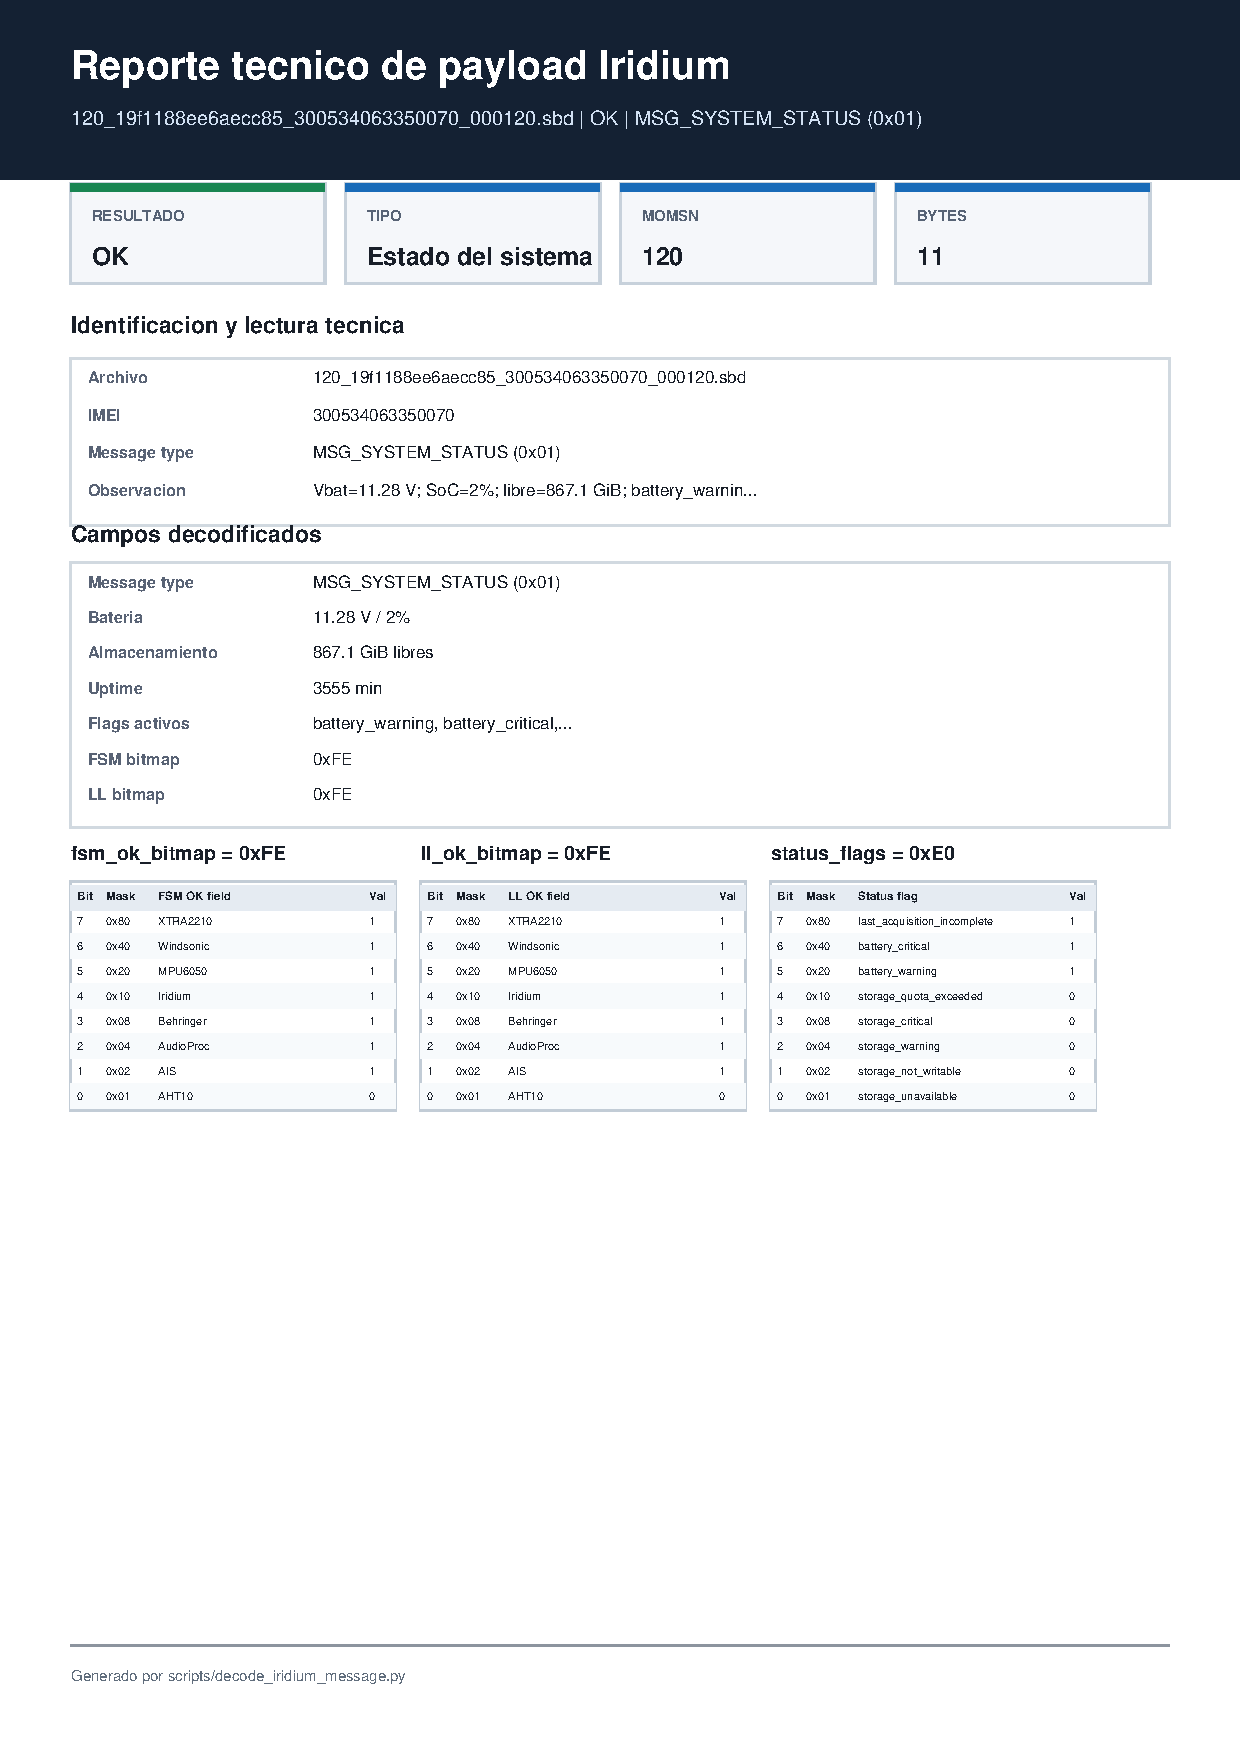
\includepdf[pages=-,scale=0.95,pagecommand={\thispagestyle{plain}}]{graficos/120_19f1188ee6aecc85_300534063350070_000120.pdf}

\clearpage

\subsection{Reporte de payload Iridium MOMSN 123}
\label{ap:reporte_sbd_momsn_123}

El reporte incluido a continuación documenta la decodificación del payload MOMSN~123 como mensaje \texttt{MSG\_AUDIO}, incluyendo cantidad de canales, cantidad de bandas, tipo de empaquetado, verificación CRC y valores de potencia relativa por banda.

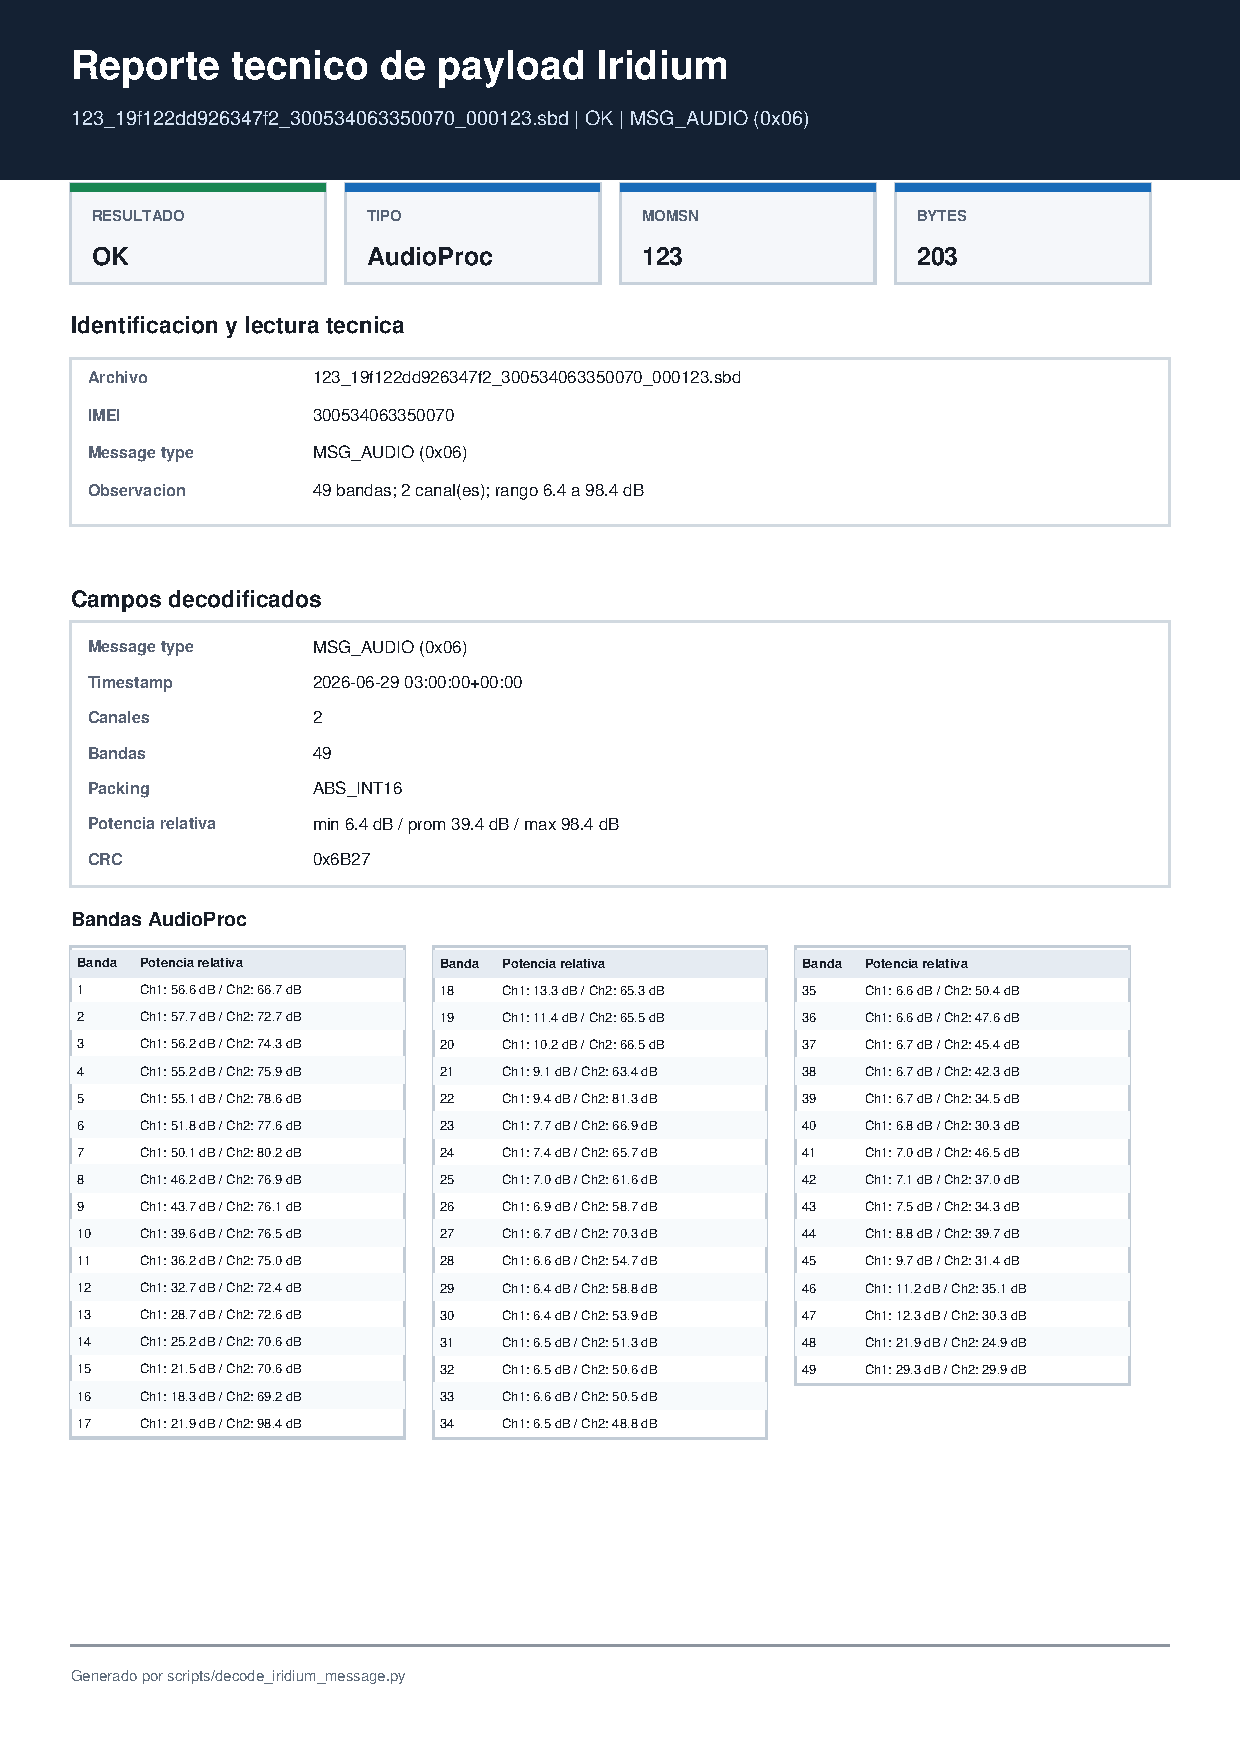
\includepdf[pages=-,scale=0.95,pagecommand={\thispagestyle{plain}}]{graficos/123_19f122dd926347f2_300534063350070_000123.pdf}

\clearpage

\subsection{Reporte consolidado de decodificación de payloads}
\label{ap:reporte_payloads_iridium}

El reporte incluido a continuación resume la corrida de decodificación aplicada al conjunto de payloads compatibles con el protocolo vigente. Este documento registra la cantidad total de archivos procesados, la ausencia de errores de decodificación, la distribución por tipo de mensaje y los rangos principales observados para los productos de AudioProc.

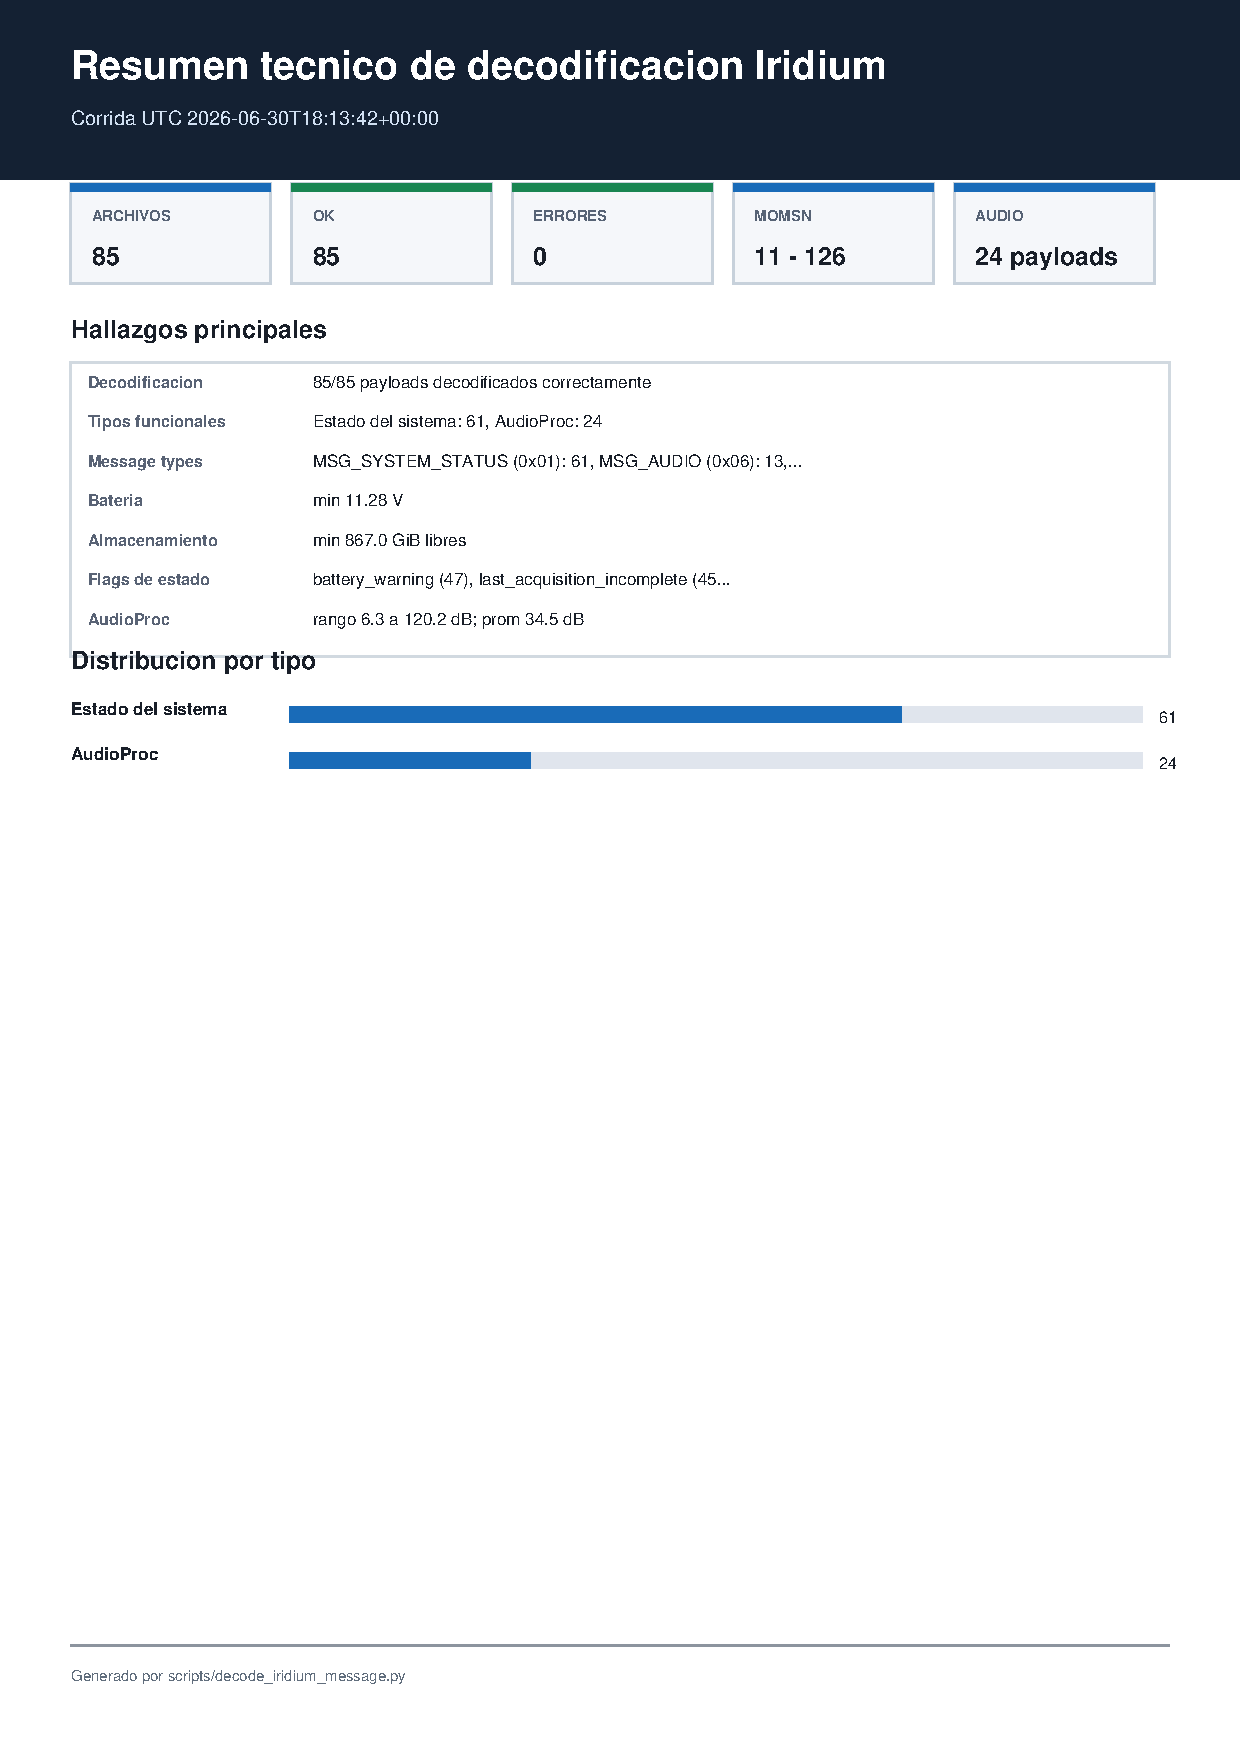
\includepdf[pages=-,scale=0.95,pagecommand={\thispagestyle{plain}}]{graficos/payloads_report.pdf}



\end{document}
